%%%%%%%%%%%%%%%%%%%%%%%%%%%%%%%%%%%%%%%%%%%%%%%%%%%%%%%%%%%%%%%%%%%%%%%%%%%%
% AGUtmpl.tex: this template file is for articles formatted with LaTeX2e,
% Modified March 2013
%
% This template includes commands and instructions
% given in the order necessary to produce a final output that will
% satisfy AGU requirements.
%
% PLEASE DO NOT USE YOUR OWN MACROS
% DO NOT USE \newcommand, \renewcommand, or \def.
%
% FOR FIGURES, DO NOT USE \psfrag or \subfigure.
%
%%%%%%%%%%%%%%%%%%%%%%%%%%%%%%%%%%%%%%%%%%%%%%%%%%%%%%%%%%%%%%%%%%%%%%%%%%%%
%
% All questions should be e-mailed to latex@agu.org.
%
%%%%%%%%%%%%%%%%%%%%%%%%%%%%%%%%%%%%%%%%%%%%%%%%%%%%%%%%%%%%%%%%%%%%%%%%%%%%
%
% Step 1: Set the \documentclass
%
% There are two options for article format: two column (default)
% and draft.
%
% PLEASE USE THE DRAFT OPTION TO SUBMIT YOUR PAPERS.
% The draft option produces double spaced output.
%
% Choose the journal abbreviation for the journal you are
% submitting to:

% jgrga JOURNAL OF GEOPHYSICAL RESEARCH
% gbc   GLOBAL BIOCHEMICAL CYCLES
% grl   GEOPHYSICAL RESEARCH LETTERS
% pal   PALEOCEANOGRAPHY
% ras   RADIO SCIENCE
% rog   REVIEWS OF GEOPHYSICS
% tec   TECTONICS
% wrr   WATER RESOURCES RESEARCH
% gc    GEOCHEMISTRY, GEOPHYSICS, GEOSYSTEMS
% sw    SPACE WEATHER
% ms    JAMES
% ef    EARTH'S FUTURE
%
%
%
% (If you are submitting to a journal other than jgrga,
% substitute the initials of the journal for "jgrga" below.)

\documentclass[jgrga, draft]{agutex}
% \documentclass[jgrga]{agutex}
% To create numbered lines:

% If you don't already have lineno.sty, you can download it from
% http://www.ctan.org/tex-archive/macros/latex/contrib/ednotes/
% (or search the internet for lineno.sty ctan), available at TeX Archive Network (CTAN).
% Take care that you always use the latest version.

% To activate the commands, uncomment \usepackage{lineno}
% and \linenumbers*[1]command, below:

\usepackage{lineno}
\linenumbers*[1]

%  To add line numbers to lines with equations:
%  \begin{linenomath*}
%  \begin{equation}
%  \end{equation}
%  \end{linenomath*}
\usepackage{amsmath}
%%%%%%%%%%%%%%%%%%%%%%%%%%%%%%%%%%%%%%%%%%%%%%%%%%%%%%%%%%%%%%%%%%%%%%%%%
% Figures and Tables
%
%
% DO NOT USE \psfrag or \subfigure commands.
%
%  Figures and tables should be placed AT THE END OF THE ARTICLE,
%  after the references.
%
%  Uncomment the following command to include .eps files
 % \usepackage[pdflatex]{graphicx}
 \usepackage{graphicx}
 \DeclareGraphicsExtensions{.pdf, .png, .jpg, .eps}
 \graphicspath{ {./figs/} }

%
%  Uncomment the following command to allow illustrations to print
%   when using Draft:
 \setkeys{Gin}{draft=false}
%
% Substitute one of the following for [dvips] above
% if you are using a different driver program and want to
% proof your illustrations on your machine:
%
% [xdvi], [dvipdf], [dvipsone], [dviwindo], [emtex], [dviwin],
% [pctexps],  [pctexwin],  [pctexhp],  [pctex32], [truetex], [tcidvi],
% [oztex], [textures]
%
% See how to enter figures and tables at the end of the article, after
% references.
%
%% ------------------------------------------------------------------------ %%
%
%  ENTER PREAMBLE
%
%% ------------------------------------------------------------------------ %%

% Author names in capital letters:
\authorrunninghead{HAMMAN ET AL.}

% Shorter version of title entered in capital letters:
\titlerunninghead{LAND-OCEAN COUPLING IN RASM}

%Corresponding author mailing address and e-mail address:
\authoraddr{Corresponding author: Bart Nijssen,
Department of Civil \& Environmental Engineering, Box 352700,
University of Washington, Seattle, WA 98195-2700, USA.
(nijssen@uw.edu)}

\begin{document}

%% ------------------------------------------------------------------------ %%
%
%  TITLE
%
%% ------------------------------------------------------------------------ %%


\title{Land-Ocean Coupling in the Regional Arctic System Model}

%% ------------------------------------------------------------------------ %%
%
%  AUTHORS AND AFFILIATIONS
%
%% ------------------------------------------------------------------------ %%


% Use \author{\altaffilmark{}} and \altaffiltext{}

% \altaffilmark will produce footnote;
% matching \altaffiltext will appear at bottom of page.

\authors{Joseph Hamman\altaffilmark{1},
Bart Nijssen\altaffilmark{1},
Andrew Roberts\altaffilmark{2},
Anthony Craig\altaffilmark{2},
Wieslaw Maslowski\altaffilmark{2},
and Robert Osinski\altaffilmark{3}}

\altaffiltext{1}{Department of Civil \& Environmental Engineering,
University of Washington, Seattle, WA, USA.}
\altaffiltext{2}{Department of Oceanography, Naval Postgraduate School,
Monterey, CA, USA.}
\altaffiltext{3}{Polish Institute of Oceanology, Sopot, Poland.}


%% ------------------------------------------------------------------------ %%
%
%  ABSTRACT
%
%% ------------------------------------------------------------------------ %%

% >> Do NOT include any \begin...\end commands within
% >> the body of the abstract.

\begin{abstract}
TODO:
% The purpose of the abstract is twofold: (1) state the nature of the investigation and (2) summarize the important conclusions of this investigation. The abstract should be suitable for separate publication in an abstract journal and be adequate for indexing. Make sure to check for the following:
%
% It is set as a single paragraph.
% It is limited to 250 words for all journals except GRL where the limit is 150 words.
% It does not include table or figure mentions.
% If it has reference citations that are part of the sentence, they should be in roman type and have parentheses around the year; parenthetical reference citations will be deleted.
% All abbreviations used in the abstract are defined.
\end{abstract}

%% ------------------------------------------------------------------------ %%
%
%  BEGIN ARTICLE
%
%% ------------------------------------------------------------------------ %%

% The body of the article must start with a \begin{article} command
%
% \end{article} must follow the references section, before the figures
%  and tables.

\begin{article}

%% ------------------------------------------------------------------------ %%
%
%  TEXT
%
%% ------------------------------------------------------------------------ %%

\section{Introduction}

% BN: I am more used to seeing a paragraph like this at the end of the introduction rather than at the beginning. It is probably just a matter of what I am used to rather than what is better, but it comes over as rather abrupt to me. Leave as is for now, but we may move it down later. (20 years ago we would never use "we" or "I" in a paper, which is clearly also a style element that has changed).
We have implemented the RVIC river routing scheme within the recently developed Regional Arctic System Model (RASM) \citep{Hamman_2016} to represent the streamflow flux between the land and ocean model components.
In this paper, we introduce the RVIC streamflow routing model and describe its coupling within RASM.
We evaluate the performance of RVIC in fully-coupled RASM simulations by comparing model simulated streamflow to in-situ observations.
We then use a sensitivity experiment in fully-coupled RASM to highlight the role and importance of accurately representing streamflow in coupled climate simulations in the Arctic.

Approximately 11\% of the global terrestrial runoff drains into the Arctic Ocean, which holds only 1\% of the Earth's salt water \citep{Lewis_2000,Lammers_2001}.
As a result, the Arctic Ocean has the lowest salinity levels among the Earth's oceans \citep{Steele_2001}.
Streamflow is the largest contributor of freshwater to the Arctic Ocean and comprises approximately 38\% of the total freshwater flux entering the Arctic Ocean; the remainder of which consists of precipitation (24\%) over the Arctic Ocean \citep{Serreze_2006} and inflow from the Pacific and Atlantic Oceans.
The streamflow contribution has a distinct seasonal cycle.
During the spring and summer months, the fractional contribution of freshwater to the Arctic from streamflow is much larger than 38\%.
% It would be great to have a actual number here. ROBERT: it would be great if we can get together on the annual and seasonal freshwater budget in RASM.
Across the Arctic region, the annual runoff hydrograph is characterized by a prominent spring freshet, with approximately 60\% of the annual runoff volume occurring between April and July \citep{Lammers_2001}.
The seasonal freshwater flux from the land to the ocean plays an important role in coastal ocean dynamics and hydrography, as well as in sea ice formation and melt \citep{Rabe_2011,Fichot_2013}.
Runoff from Arctic river basins is the primary source of buoyancy-driven currents such as the Alaska, Siberian, Norwegian, and East Greenland coastal currents \citep[e.g.][]{Morison_2000,Boyd_2002,McGeehan_2012}.
These currents redistribute both fresh water and heat, which locally play important roles in shelf dynamics and shelf-basin interactions.
Buoyancy delivered by rivers also affects the onset of sea ice formation in winter and melt in spring and summer.
Water with lower salinity freezes at higher temperatures, and therefore does not have to be cooled as much as higher salinity water to freeze.
Thus, for a warming and freshening Arctic Ocean, the onset of freezing may be partially buffered against regional warming in areas highly influenced by streamflow.
However, the earlier sea ice freeze-up enabled by low sea surface salinity (SSS) also reduces the amount of heat the upper ocean can lose in the fall, counteracting the impact freshening has on sea ice development \citep{Morison_2012}.

In the long-term, river runoff balances freshwater export through Fram Strait and the Canadian Arctic Archipelago into the North Atlantic and consequently maintains the surface freshwater layer in the Arctic Ocean, which is important for maintaining the stratification of the Arctic Ocean \citep{Nummelin_2015}. % BN: Is there no freshwater export into or import from the North Pacific?  --- JJH: There is net import through the Baring Strait.
Although warmer, less dense water exists at depth in the Arctic Ocean, stratification is maintained by the density gradient between the cold fresh mixed layer above and the more saline halocline and Atlantic water layers below \citep{Serreze_2006}.
These stratifying processes limit the heat flux into the mixed layer from below.

% [ocean / sea ice specific studies]
The terrestrial freshwater flux has been shown to be an important driver of ice-ocean dynamics in coupled ice-ocean models \citep[e.g.][]{Morison_2012,Lique_2015,Large_2009}.
\citet{Newton_2008} applied observed climatological runoff from nine of the largest rivers within the Arctic basin in the Naval Postgraduate School (NPS) Arctic regional Model (NAME).
Their study used passive Lagrangian flow tracers within their model to track the spatial distribution of runoff.
They found the highest concentrations of river runoff along the Siberian coast.
Despite our understanding of the importance of river runoff in Arctic Ocean dynamics, \citet{Nummelin_2015} show that global climate models [GCMs] poorly represent the vertical structure of the Arctic Ocean, with many models failing to accurately reproduce the observed profiles of temperature and salinity in the upper 500 m.
They conclude that a correct representation of the streamflow flux is a key step toward improving the performance of the ocean model components in these models.
\textit{All - if there are other relevent studies that have explored the role of streamflow on regional or global ocean dynamics, please let us know}

Numerous observational and modeling studies have explored the seasonal and inter-annual behavior of Arctic runoff. % BN: We should include a brief mention and description of the CORE2 data set, since it appears to be widely used withing the arctic science community
\citet{Lammers_2001} compiled the R-ArcticNET database, a regional hydrographic record of mean monthly streamflow observations that includes over 3,700 streamflow gauges in the Pan-Arctic region.
The collection of observations in R-ArcticNET was later used by \citet{Shiklomanov_2009} in their investigation of increasing river discharge in the largest Eurasian rivers and by \citet{Tan_2011} in their study of changes in spring snowmelt timing.
\citet{Dai_2009} extended portions of the R-ArcticNET database through 2007 for a subset of coastal streamflow gauges.
\citet{Adam_2007}, \citet{Adam_2008}, \citet{Su_2005}, and \citet{Dai_2009} all have used uncoupled land surface models (LSMs), in conjunction with routing schemes to simulate streamflow across the pan-Arctic region.
These studies have led to an improved understanding of the terrestrial hydroclimate in the Arctic and how the seasonal streamflow dynamics in the Arctic basin respond to changes in climate and water management activities.
However, there has not been significant research applied to understanding the role of streamflow as a coupled process in the greater Arctic climate system. % BN: Is this true? This is a potential reviewer trigger ("the authors are clearly unfamiliar with MY important work"). If we don't really need it, then I would actually delete the sentence, especially since it should become clear from the next paragraphs.

% [other climate models that include coupled land-ocean dynamics]
Cell-to-cell routing methods, such as the River Transport Model (RTM) \citep{Branstetter_2003} have been applied globally in a number of GCMs, including in the Community Earth System Model (CESM).
These cell-to-cell models are typically difficult to parameterize across a range of spatial scales \citep{Sushama_2004}.
Source-to-sink routing models \citep[e.g.][]{Lohmann_1996,Naden_1992}, akin to the RVIC model used in this study, have also been previously applied in coupled models \citep[e.g.][]{Olivera_2000}.
Source-to-sink routing methods do not explicitly track streamflow between grid cells; rather, they parameterize the distribution and travel time of runoff between source and outlet grid cells.
In previous applications of source-to-sink routing models within coupled climate models \citep[e.g.][]{Olivera_2000}, the streamflow routing has been applied at coarse spatial resolutions (greater than 200 km) and low frequency coupling (e.g. daily).
Furthermore, these studies have typically focused on global applications and have not specifically evaluated the importance of streamflow in terms of coupled land-ocean interactions.
In recent years, there have been fewer studies of developing or evaluating streamflow routing schemes coupled within earth system models. % BN: But there has been significant work in the development of regional- and global-scale routing models of increasing complexity. For example, MOSART, the model from Yamazaki (e.g. doi:10.5194/hess-13-2241-2009, doi:10.1002/2014GL059744), and mizuRoute (doi:10.5194/gmd-9-2223-2016). We need to reference that literature.
\citet{Bring_2015}, in their recent synthesis of CMIP5 runoff dynamics, conclude that a significant community effort should be made to improve the understanding and modeling of basin scale freshwater fluxes in coupled climate modeling.
This argument is further echoed by \citet{Lique_2015} in their recent review paper on the representation of the Arctic hydrologic cycle in coupled climate models.

In this paper, we describe the land to ocean coupling in the Regional Arctic System Model.
We introduce the RVIC streamflow routing model in Section \ref{sec:models}, detailing its coupling within RASM.
We describe the model simulations and observed data that we have used in Section \ref{sec:data}.
In Section \ref{sec:results}, we present results from fully-coupled RASM simulations where the land and ocean are coupled via the runoff flux.
We compare simulated streamflow to observations at gauging locations and explore the role of the terrestrial freshwater flux in the ice and ocean components within RASM.
Section \ref{sec:discussion} includes a discussion on the role of streamflow in the Arctic climate system and the scientific advances and drawbacks associated using a source-to-sink routing model such as RVIC.
Finally, in Section \ref{sec:conclusions}, we provide our conclusions and highlight the potential for further research using the RVIC model.

\section{Models}
\label{sec:models}

\subsection{RASM}
\label{sec:rasm}
The Regional Arctic System Model is a fully coupled, high spatial and temporal resolution regional earth system model applied over the pan-Arctic domain.
Principal goals of the modeling project are to better understand the interaction between physical systems in the Arctic drainage basin, to advance understanding of past and present states of Arctic climate, and to improve seasonal to multi-decadal prediction capabilities of key Arctic indicators.
Model components are coupled using the CESM coupled model framework and the CPL7 flux coupler \citep{Craig_2011}.
Below, we provide a brief description of the five component models in RASM version 1.0 (Figure \ref{fig:rasm_schematic_domain}a).
For the purposes of this paper, we are principally concerned with the coastal streamflow flux and its role in the Arctic Ocean system and our description below  focuses on the streamflow and ocean model components.
The reader will find additional information on the implementation of individual component models in the RASM-specific references cited below.

\begin{enumerate}
\item CICE: The Los Alamos Sea Ice model is a physically-based, dynamic sea ice model \citep{Hunke_2010}.
\citet{Roberts_2015a} provide a description of the application of CICE, version 5, within RASM.
\item POP: The Parallel Ocean Program model is a general circulation ocean model \citep{Smith_2010}.
\citet{Roberts_2015a} provide a description of the application of POP, version 2, within RASM.
Of particular relevance to this study, POP uses a virtual salinity flux to represent changes in ocean salinity due to surface fluxes of freshwater (runoff, precipitation, and evaporation).
The virtual salt flux ($VSF$) is calculated as
\begin{equation}
  \label{eq:SaltFlux}
  VSF= -F_w S
\end{equation}

where $F_w$ is the sum of the freshwater fluxes from streamflow, precipitation, evaporation, and sea ice melting and freezing. $S$ is reference salinity, which is the surface salinity of the grid cell where input of fresh water is taking place. % BN: How is this reference salinity prescribed or determined?

\item VIC: The Variable Infiltration Capacity model \citep{Liang_1994} is a macroscale land surface hydrology model.
\citet{Hamman_2016} provide a description of the application of VIC within RASM.
\item WRF: The Weather Research and Forecasting atmospheric model \citep{Skamarock_2007} is a mesoscale meteorological model.
\citet{Cassano_2016} provide a detailed description of the WRF model, version 3.2, as it is applied in RASM.
\item RVIC: The RVIC streamflow routing model is an adapted version of the \citet{Lohmann_1996} linear, source-to-sink routing model frequently used to route the runoff flux from the VIC model.
A complete description of the RVIC model is provided in Section~\ref{sec:rvic}.
\end{enumerate}

In RASM Version 1.0, the land, atmosphere, and runoff components share a 50-km near-equal-area North Pole stereographic grid mesh.
The ocean and sea ice models share a 1/12$^{\circ}$ rotated stereographic grid mesh (Figure \ref{fig:rasm_schematic_domain}b).
All model components are coupled every 20 minutes.
This coupling configuration is described by \citet{Roberts_2015a}, where the sub-daily coupling frequency is shown to be important in reproducing observed inertial frequencies in the atmosphere-ice-ocean coupling cycle.

\subsection{RVIC}
\label{sec:rvic}

The RVIC streamflow routing model is a modified version of the routing model typically used to post-process VIC model output \citep{Lohmann_1996, Lohmann_1998a}.
The original \citet{Lohmann_1996} model has been used in many offline modeling studies from regional to global spatial scales at horizontal resolutions from 1/16$^{\circ}$ to 2$^{\circ}$ \citep[e.g.][]{Nijssen_1997,Lohmann_1998b,Su_2005,Hamlet_2013}.
RVIC is a source-to-sink routing model that solves a linearized version of the Saint-Venant equations \citep{Fread_1992,Mesa_1986}.
The linearized Saint-Venant equations (\ref{eq:St_Venant}) are a one-dimensional model describing unsteady flow in terms of two time-invariant parameters, flow velocity and diffusivity.
The velocity and diffusivity parameters can be estimated from observed streamflow, through numeric optimization, or by solving the Saint-Venant equations directly. % BN: But if you already solve the S-V equations directly, why would you need RVIC?
RVIC uses flow direction raster (FDR) grids, typically derived from topographic information \citep[e.g.][]{Wu_2011}, to specify the flow path and distance for each source-sink pair.
The flow along the travel path is parameterized as a linear time-invariant unit impulse response function (IRF) to runoff generated at individual grid cells by the LSM, often referred to as a unit hydrograph (UH).
The application of the RVIC model has two distinct steps, a preprocessing step in which IRFs are developed for each source-toink pair (see Sections ~\ref{sec:irfs} and ~\ref{sec:remap}), and a computationally efficient convolution step in which distributed runoff from the LSM is routed to downstream points (see Section~\ref{sec:convolution}).

The RVIC model differs from the original \citet{Lohmann_1996} model in four main ways:

\begin{enumerate}
\item RVIC completely separates the development of the IRFs from the flow convolution step,
\item RVIC allows the development of the IRFs to be done on flow direction grids that do not match the grid elements used for the land model (see Section~\ref{sec:irfs}),
\item The RVIC convolution scheme operates in a space-before-time pattern, facilitating direct coupling with LSMs (see Section~\ref{sec:convolution}),
\item RVIC includes numerous infrastructure improvements, including parallel processing, the ability to store the exact model state, and to read and write netCDF files.
\end{enumerate}

The stand-alone version of the RVIC model, complete with documentation and example input data, is available via a publicly accessible source code repository \citep{Hamman_2015}.

\subsubsection{Impulse response function development}
\label{sec:irfs}

A unit hydrograph describes the streamflow response of an area (e.g. basin or grid cell) to a unit input of runoff ($Q^F$) in terms of timing and volume (see Figure \ref{fig:uh_remap_schematic}-c).
The development of the IRF for every source-to-sink pair is a combination of a UH describing lumped routing behavior of streamflow within the source grid cell plus the horizontal travel to the downstream point with the addition of a flow diffusivity parameter.
The horizontal travel path and distance are computed using a flow direction raster \citep[e.g.][]{Wu_2011}.
The Saint-Venant equation is given by

 \begin{equation}
   \label{eq:St_Venant}
   \frac{\partial Q}{\partial t} = D \frac{\partial^2 Q}{\partial x} + C \frac{\partial Q}{\partial x}
 \end{equation}

where $Q$ represents the flow at time $t$ at a downstream point $x$ as a function of the wave velocity $C$ and the diffusivity $D$; both of which may be estimated from geographical data. Eq.~(\ref{eq:St_Venant}) can be linearized and solved with convolution integrals

 \begin{equation}
   \label{eq:conv_integral}
	  Q(x,t) = \int_0^t UH(t-s)h(x,s)ds
 \end{equation}

where

 \begin{equation}
   \label{eq:Greens_IRF}
	h(x, t) = \frac{x}{2t\sqrt{\pi tD}}exp\left(-\frac{(Ct-x)^2}{4Dt}\right)
 \end{equation}

is a Green's impulse response function, and $UH$ is a unit hydrograph representing the distribution of flow from within each source grid cell to the edge of the source grid cell.
Equations \ref{eq:conv_integral} and \ref{eq:Greens_IRF} are solved to determine the flow response for each source-to-sink pair.

\subsubsection{Upscaling and basin aggregation}
\label{sec:remap}

The original employment of the \citet{Lohmann_1996} model required that the flow direction grid and the LSM grid match exactly.
This limited the applicability of the model and required either the LSM to be evaluated on the same grid as an existing flow direction dataset grid or the custom generation of a flow direction grid for each LSM grid.
The RVIC implementation allows the development of the IRFs on a different grid, usually higher spatial resolution, than the LSM by upscaling and aggregating the high resolution IRF grid to the LSM grid (Figure \ref{fig:uh_remap_schematic}).
The upscaling process uses the first-order conservative remapping technique developed by \citet{Jones_1999}. % BN: You are never specific on what you are remapping. This section needs a little more detail to be understandable by people not directly familiar with what we are trying to do
Because the remapping scheme is conservative, each of the resulting IRFs on the LSM grid are an area weighted average of the IRFs on the high resolution FDR  grid.
Finally, in the event there are multiple sink points on the FDR grid within a single LSM grid cell, the upscaled IRFs are combined to include all source points flowing into a single outlet grid cell.

\subsubsection{Convolution}
\label{sec:convolution}

The convolution step combines the IRFs with the discharge fluxes from the LSM.
The streamflow $Q$ for each outlet grid cell $x$ and time $t$ is given by

\begin{equation}
  \label{eq:convolution}
   Q(x,t) = \int_0^{S(x)} \int_0^{\infty}\,IRF(s,t)\,Q^F(s,t-\tau)\,d\tau\,ds
 \end{equation}

where $S(x)$ is the number of source ($s$) grid cells, and $\tau$ is the position in the IRF vector.
RVIC's application of the convolution is practically equivalent to the one described by \citet{Lohmann_1996}.
The key difference is in the implementation, where the time integral has been moved to the outer loop in RVIC, allowing for stepwise evaluation of the convolution over the entire spatial model domain.

\subsubsection{RVIC in RASM}

The IRFs used in RASM were developed using the 1/16$^{\circ}$ FDRs from \citet{Wu_2011}.
RVIC in RASM uses a spatially constant flow velocity and diffusivity of 0.6 m/s and a 3,000 m$^2$/s, respectively.
These parameters were chosen using the calibration methods described in Section~\ref{sec:parameters} and fit within the valid ranges for these parameters discussed in the literature \citep[e.g.][]{Decharme_2010,Lohmann_1996}.
Hourly IRFs were developed for each of the 95,001 coastal 1/16$^{\circ}$ grid cells bordering the ocean model and were upscaled and aggregated to the 4,841 coastal grid cells on the 50-km near equal area land surface grid that is used by RASM version 1.0.

Turbulent mixing and other diffusive processes combine to gradually spread fresh water along the coast and into the open ocean. % BN: Is the same method used in CESM or other models? If so, is there a reference we can include?  --- JJH: Good question, I asked Tony this when he sent me this description and he said there was not, to his knowledge, a reference to cite.
In a coupled modeling environment however, these processes are difficult to represent at the spatial scales at which the runoff, ocean, and sea ice models are configured.
To simulate the dispersion of fresh water throughout each ocean grid cell within RASM, a diffusion scheme is applied within the coupler (CPL7) to avoid unrealistic salinity gradients that could occur where a river's entire outflow is applied to a single ocean grid cell.
The mapping from the runoff grid to the ocean grid is generated as a preprocessing step using the runoff and ocean grids.
Each runoff gridcell is mapped to the nearest ocean grid cell.
The flux is then smoothed over all grid cells in a 300 km radius ($r_{max}$) with a distance ($r$) weighted logarithmically decreasing e-folding scale of 1000 km ($r_{fold}$) such that the total quantity is conserved from runoff to ocean. % BN: We need to standardize on "name (symbol)" or "name symbol". Since the typography is different for name and symbol, I am fine with either, as long as we are consistent
The mapping weights $w(r)$ are given by

\begin{equation}
  \label{eq:diffusion}
  w(r)=
     \begin{cases}
        e^{(-r/r_{fold})} & 0\leq r\leq r_{max} \\
        0 & r > r_{max}
     \end{cases}
\end{equation}

\subsection{Parameter Selection}
\label{sec:parameters}

We used a brute force parameter evaluation procedure to select the velocity and diffusivity parameters for the RVIC model applied in RASM.
For this procedure, RVIC was run offline (i.e. not coupled to RASM) at a daily timestep and was forced using daily runoff fluxes from the fully coupled RASM simulation described as $RASM_{ERA}$ in \citet{Hamman_2016}.
These runoff fluxes include both the fast-reponse and slow-response runoff components generated by the LSM.
The velocity parameter was varied between 0.2 and 1.5 m/s and the diffusivity was varied between 500 and 4,000 m\textsuperscript{2}/s. % BN: Is there a reason for these parameter bounds?
Individual pairs of parameters were evaluated using a modified version of the overlap statistic \citep{Perkins_2007} as the objective function.
The overlap statistic, which was originally introduced as a measure of likeness for probability density functions, is applied here to the normalized mean monthly hydrographs of the six largest river basins in the RASM model domain (Figure \ref{fig:rasm_schematic_domain}b).
The overlap statistic is perhaps the best performance measure of the routing model because it focuses entirely on the shape of the hydrograph and does not take the bias in the flow volume into account (Figure \ref{fig:calibration_hydrographs}). This is desirable since the volume bias is determined by the LSM (and the other components in a coupled model environment) and not affected by the routing model which is mass-conserving.
The final velocity and diffusivity parameters, 0.6 m/s and 3,000 m\textsuperscript{2}/s, respectively, were chosen to maximize the composite overlap statistic for the six largest rivers in the RASM domain, where the composite was formed by weighting each basin's overlap statistic by that basin's runoff volume (Figure \ref{fig:calibration_hydrographs}).

\section{Model Simulations and Data}
\label{sec:data}

We present results from two fully-coupled RASM simulations, $RASM_{CONTROL}$ and $RASM_{NOROF}$, using RASM version 1.0 (Tag R1010), each using ERA-Interim boundary conditions.
We also highlight the impact of the calibration procedure with an offline RVIC simulation, $RVIC_{FAST}$, forced with VIC discharge from $RASM_{CONTROL}$.
All three simulations were run from September 1, 1979 through December 31, 2009.
For the RASM simulations, we focus our analysis on the period January 1, 1990 through December 31, 2009, allowing for a 10 year model spin-up of the coupled system.
Both RASM simulations began with the same initial state \citep[see][]{Hamman_2016} and use identical land, atmosphere, ocean, and sea ice model configurations.
These simulations only differ as follows:
\begin{itemize}
     \item $RASM_{CONTROL}$: uses the calibrated RVIC parameters described above.
     \item $RASM_{NOROF}$: does not include the runoff flux from the land to the ocean.
     \item $RVIC_{FAST}$: stand-alone RVIC simulation forced with $RASM_{CONTROL}$.
          This simulation uses velocity and diffusivity parameters of 2.0 m/s and 2,000 m\textsuperscript{2}/s, respectively.
          These parameter values are frequently used as the default values with the RVIC model and were the original values used when developing RVIC within the coupled model. % BN: Figure out how to indent a multi-line item properly. There must be an easy way to do this, but a 2-minute search did not give me what I needed
          % BN: I would move the motivation for these "default" values to the previous section
\end{itemize}

We compare output from RASM simulations to streamflow observations in the \citet{Dai_2009} dataset, hereafter referred to as D2009. % BN: I'd prefer to the values as D2009 rather than observations, to make it clear that this dataset also involves some manipulation of the (limited) observations that exist.
This dataset provides mean monthly streamflow observations at the most downstream gauging location for more than 60 individual river basins within the RASM domain and analysis period. % BN: Provide a little more info (1-2 lines) on the background of the Dai dataset, since that is what we are comparing against. How much of that is observations versus models? Why not use R-ArcticNet directly? Why not use Core2? -- but keep it short.

\section{Results}
\label{sec:results}

\subsection{Streamflow Hydrographs}
\label{sec:hydrographs}

% BN: I suggest that you restructure this section. As is, the sequence is awkward. You discuss RASM_control first and then RVIC_fast, but since RASM_control is much better it is unclear why you would ever be interested in RVIC_fast. However, if you treat RVIC_fast as the a priori, pre-calibration setup and discuss that, then it motivates the parameter selection process and demonstrates the improvement that can be made through parameter optimization (and it also shows the limits of that method since you cannot affect the volume that way)
Our analysis of the streamflow hydrograph extends the results of \citet{Hamman_2016} to the monthly timestep.
Figure \ref{fig:hydrographs} compares the monthly hydrographs for $RASM_{CONTROL}$ and $RVIC_{FAST}$ at the six streamflow gauge locations shown in Figure \ref{fig:calibration_hydrographs}.
These hydrographs are compared to values from D2009 for the period 1990 to 2006.
The annual overlap, and monthly RMSE statistics for these six monthly hydrographs are shown in Table \ref{table:rivers}. % BN: The bias is not interesting since you already explained that this is not governed by the routing model. If you do include it, then I would not include two separate columns for the two different routing runs, but just use one column to avoid confusion (the small differences are meaningless and simply round-off or start and end effects)
The $RASM_{CONTROL}$ hydrographs in the Amur, Lena, and Yukon basins match D2009 best, with overlap statistics between 0.79 and 0.9.
In the Ob, Yenisey, and Mackenzie River basins, the $RASM_{CONTROL}$ streamflow shows positive biases in the winter and spring and negative biases in the summer.
Consequently, the overlap statistic for these rivers is lower ($<$ 0.75).
In these basins, during the winter, it is clear that VIC is underestimating the baseflow flux.
For most of the basins shown in Figure \ref{fig:hydrographs}, the timing of the peak month in the $RASM_{CONTROL}$ simulation occurs one month before the observations.
This peak streamflow timing bias is likely due to a spring and summer warm bias in the $RASM_{CONTROL}$ simulation \citep{Hamman_2016,Cassano_2016}, resulting in premature snow melt and runoff.
The notable exception to this is in the Ob River basin, where the runoff regime is acutely influenced by extensive wetlands and permafrost, and the spring peak occurs a month early in $RASM_{CONTROL}$ (May vs. June).
Compared to the normalized hydrographs in Figure \ref{fig:calibration_hydrographs}, the majority of the disagreement in Figure \ref{fig:hydrographs} is due to the bias in the total annual runoff flux which is not contolled by the mass conserving RVIC routing model.
\citet{Hamman_2016} provide a more detailed, intermodel comparison of the annual runoff biases in the Arctic and find that the performance of the VIC LSM is as good or better than other coupled models.

The peak spring freshet in $RVIC_{FAST}$ occurs about one month earlier than in $RASM_{CONTROL}$.
On average, this leads to values for the overlap statistic that are about 15\% lower than for the $RASM_{CONTROL}$ simulation.
The differences in the routing parameters used in the $RASM_{CONTROL}$ and $RVIC_{FAST}$ simulations can be clearly identified in the annual cycle column of Figure \ref{fig:hydrographs}.
The bias in timing of the peak spring freshet is mostly due to the difference in streamflow velocity (2.0 vs. 0.6 m/s), whereas the shape of the hydrograph is largely determined by the diffusivity parameter (2000 vs. 6000 m\textsuperscript{2}/s).

Figure \ref{fig:taylor} shows a Taylor Diagram comparing the RASM simulated hydrographs at 64 observation locations.
The Taylor Diagram shows the correlation along the arc and the normalized standard deviation ratio along the radius.
The contours denote lines of equal root-mean-square error (RMSE) where a correlation of 1.0 and a standard deviation ratio of 1.0 represent a RMSE of zero.
While the correlation coefficients in $RVIC_{FAST}$ are not distributed according to the flow magnitude, the largest basins in $RASM_{CONTROL}$ tend to perform better with correlation coefficients typically increasing by about 0.3.
This is likely due to our choice to calibrate the runoff parameters using only the largest basins in the domain. % BN: I don't know what you mean by: "The correlation coefficients are not distributed according to the flow magnitude"
While the correlations are shown to improve in nearly all of the basins in Figure \ref{fig:taylor}, the standard deviations are not shown to be significantly impacted by the calibration.
This indicates that the variability in the monthly timeseries is not significantly controlled by the routing model and is more a function of the runoff flux coming from the LSM.

\subsection{Role of high resolution coastal streamflow on ocean and sea ice dynamics}
\label{sec:ocean}

Figure \ref{fig:ocean_timeseries} shows the timeseries of streamflow for the Central Arctic and greater POP domain.
In the Central Arctic basin, melt season streamflows can be greater than 500 km$^3$/month and nearly zero during the winter.
As discussed in Section \ref{sec:hydrographs}, the winter streamflow minimum is likely underestimated in RASM due to cold season biases in the baseflow flux generated from VIC.
On an annual basis, the streamflow shown in Figure \ref{fig:ocean_timeseries} comprises approximately XX percent (ROBERT: PLEASE CALCULATE) of the total freshwater flux into the central arctic basin; 90 percent of which is delivered between May and September. % BN: Can Andrew do this?

% salinity
Figure~\ref{fig:ocean_timeseries} also shows the timeseries of SSS and sea surface temperature (SST) for the $RASM_{CONTROL}$ and $RASM_{NOROF}$ simulations.
The SSS in $RASM_{NOROF}$ is in a transient state until about the year 2000, while the $RASM_{CONTROL}$ reaches a steady state about 10 years earlier (c. 1990).
By 2010, the SSS differs in the two simulations by about 0.6 ppt (parts per thousand) for the full ocean domain and by 1.5 ppt for the central arctic basin.
The differences in the SSTs between the two simulations are relatively small when averaged over the full ocean domain, $RASM_{CONTROL}$ simulation is found to be about 0.25 $^{\circ}$C warmer than the $RASM_{NOROF}$ simulation in the central arctic basin.

% BN: The results here are a little less ambitioous than what I had hoped for. Probably mostly because of the delay on Robert's end, but I had hoped that we'd be able to show some differences in depth of the mixed layer, etc. Is there a way we can tease a little more info out of all these runs. There is a huuuge amount of computer time and effort involved here and it does not clearly show that. The Serreze schematic was nice in that regard because it pulled all the pieces together, but I understand why that will not be part of this paper.

\section{Discussion}
\label{sec:discussion}

\subsection{Impacts on the Arctic Climate System}
The largest and most direct impact that the inclusion of the streamflow flux has within the Arctic climate system is on near coastal SSS.
However, this impact on SSS is expected to translate to changes in the ocean temperature as well as the sea ice distribution.
Spatial maps of seasonally averaged SSS, SST, and sea ice height are shown in Figure \ref{fig:ocean_maps}.
While regions outside of the Central Arctic are not significantly different between the two RASM simulations, the Central Arctic basin is shown to be between 1 and 6 ppt fresher in $RASM_{CONTROL}$ than in $RASM_{NOROF}$.
The differences between the two simulations are largest in closed ocean basins (e.g. Hudson Bay) and along shallow shelfs that are adjacent to the outlets of large rivers (e.g. Siberian Shelf and Mackenzie).
Outside the Central Arctic, particularly around the margins of Greenland and in Baffin Bay, there are large areas where the salinity in $RASM_{CONTROL}$ is considerably lower than in $RASM_{NOROF}$.
In the Central Arctic, sea ice height for the $RASM_{NOROF}$ simulation is higher in all seasons by about 0.1 to more than 0.5 m, these differences are largest in the Laptav Sea.
% BN: You had made a comment the other day that the increased freshness also led to earlier freeze and that RASM nicely captured this. You mentioned this process earlier, but you do not refer to it here at all. You need to explicitly discuss that here. You need to expand this section further and compare and contrast it with results from other models / observations. As is, I am concerned that a reviewer will argue: This is great, but what is new?

\subsection{Routing Processes}

% BN: and then what would you do with it? I think you need to be clear about strengths as well as weaknesses and not only the latter.
% TODO: start this section with a description of the processes RVIC represents effectively.

While we have shown that RVIC, coupled within RASM, is able to capture the first order behavior of streamflow processes affecting the position and shape of the annual hydrograph, we know it does not include the capacity to accurately capture many of the second order processes unique to the Arctic.
For example, there is no mechanism in the RVIC model to account for non-linear routing processes such as overbank flow, wetlands, ice jams, reservoir operations, and industrial or agricultural withdrawals.
\citet{Adam_2007} highlight the importance of representing the reservoir influences in order to capture the annual hydrograph in some Eurasian rivers.
Errors caused by not explicitly representing these processes are apparent, for example, in the Nelson River (Figure \ref{fig:hydrographs}) where RVIC produces a naturalized hydrograph that bears little resemblance to the observed hydrograph which is highly influenced by reservoir operations.
Ice dam dynamics during the spring melt affect many of the high latitude rivers and are also not well represented using a linear routing model.
However, due to the timestep of the analysis here, we do not believe these processes contribute significantly to the errors in streamflow timing, nor are they likely to significantly impact the coupling with the ocean model.

While the initial implementation of the RVIC model coupled within RASM completes the freshwater cycle, it does not provide explicit mechanisms to deterministically route other runoff properties, such as heat, nutrients, or sediments.
Previous studies \citep[e.g.][]{vanVliet_2011,vanVliet_2012}, using the original \citet{Lohmann_1996} model, have included uncoupled representations of water quality and temperature.
Back of the envelope estimates of land-ocean heat flux in the Arctic, using estimated streamflow temperatures provided at a selection of rivers by \citet{Lammers_2007} have been calculated for each of the ocean basins shown in Figure \ref{fig:rasm_schematic_domain} and are provided in Table \ref{table:heat_fluxes}.
While this heat flux into the Arctic ocean is unlikely to significantly impact the regional ocean energy budget, it is likely to play an important role in the spring melt of sea ice near the outlet of large rivers.

\section{Conclusions}
\label{sec:conclusions}

The RVIC streamflow routing model is a sink-to-source river routing scheme that has been coupled within the Regional Arctic System Model, completing the hydrologic cycle between the land and ocean model components.
This paper has introduced the RVIC model, demonstrated its ability to simulate the first-order routing processes in the Arctic, and shown the relative importance of including the runoff flux in coupled ocean modeling applications.
In doing so, we conclude the following:

\begin{itemize}
\item Linear routing models, such as RVIC, can be applied within coupled model frameworks to provide high temporal and spatial frequency runoff to ocean models.
RVIC is computationally inexpensive and is relatively easy to parameterize, two features that add to its applicability in a wide range of coupled climate modeling applications.
\item Using the remapping and upscaling approach of unit hydrographs described in Section ~\ref{sec:remap}, we introduced a new method for developing unit hydrographs using dissimilar flow direction and routing grids.
Although not specifically discussed in this paper, we hypothesize that this method preserves the small scale routing behavior while facilitating routing to be done on the more coarse land surface grid. % BN: I think you can say a little more about this in the section in which you discuss upscaling the IRFs
This point warrants additional evaluation in follow-up studies.
\item The parameter selection process we have performed demonstrates that a relatively simple optimization procedure can provide significantly better routing model behavior.
Of course, a more thorough parameter selection procedure can be used in which  watersheds would be calibrated individually using distributed velocity and diffusivity parameters derived from original sources (e.g. digital elevation models).
However, the spatial and temporal scales of interest in this study did not warrant this level of optimization.
\item More complex routing schemes are likely required to adequately capture additional fluxes related to streamflow routing.
In our discussion, we have highlighted the fact that RVIC is not well positioned to handle the routing of additional quantities such as stream temperature, nutrients, or sediments.
We recognize that the representation of these quantities may be important to a range of biogeophysical processes in the near surface ocean in coupled models.
New, more complex and physically based routing models, such as the recently developed MOSART model \citep{Li_2013}, offer some potential to provide additional process representation.
The obvious challenge with these models is developing and tuning the required input parameters.
\item The presence of runoff in the RASM ocean and sea ice system has led to decreased SSS, increased SSTs, and decreased sea ice height in the Central Arctic basin.
This result partially corroborates the findings of \citep{Morison_2012} insofar as they also indicated, from an observational perspective, that a fresher Arctic Ocean would have less sea ice. % BN: Work this into the discussion as well.

\end{itemize}
%%% End of body of article:

%%%%%%%%%%%%%%%%%%%%%%%%%%%%%%%%
%% Optional Appendix goes here
%
% \appendix resets counters and redefines section heads
% but doesn't print anything.
% After typing \appendix
%
%\section{Here Is Appendix Title}
% will show
% Appendix A: Here Is Appendix Title
%
%%%%%%%%%%%%%%%%%%%%%%%%%%%%%%%%%%%%%%%%%%%%%%%%%%%%%%%%%%%%%%%%

%  ACKNOWLEDGMENTS

\begin{acknowledgments}
This research was supported under United States Department of Energy (DOE) grants DE-FG02-07ER64460 and DE-SC0006856 to the University of Washington, and XXXXXXXXXX to the Naval Post Graduate School.
Supercomputing resources were provided through the United States Department of Defense (DOD) High Performance Computing Modernization Program at the Army Engineer Research and Development Center and the Air Force Research Laboratory.
\end{acknowledgments}

%% ------------------------------------------------------------------------ %%
%%  REFERENCE LIST AND TEXT CITATIONS

\bibliographystyle{agu08}
\bibliography{biblio}

%% ------------------------------------------------------------------------ %%
%
%  END ARTICLE
%
%% ------------------------------------------------------------------------ %%
\end{article}


%% Enter Figures and Tables here:
%
% DO NOT USE \psfrag or \subfigure commands.
%
% figure captions go below the figure.
% Table titles go above tables; all other caption information
%  should be placed in footnotes below the table.
%
%----------------
% FIGURES
%

\clearpage
\begin{figure}
\noindent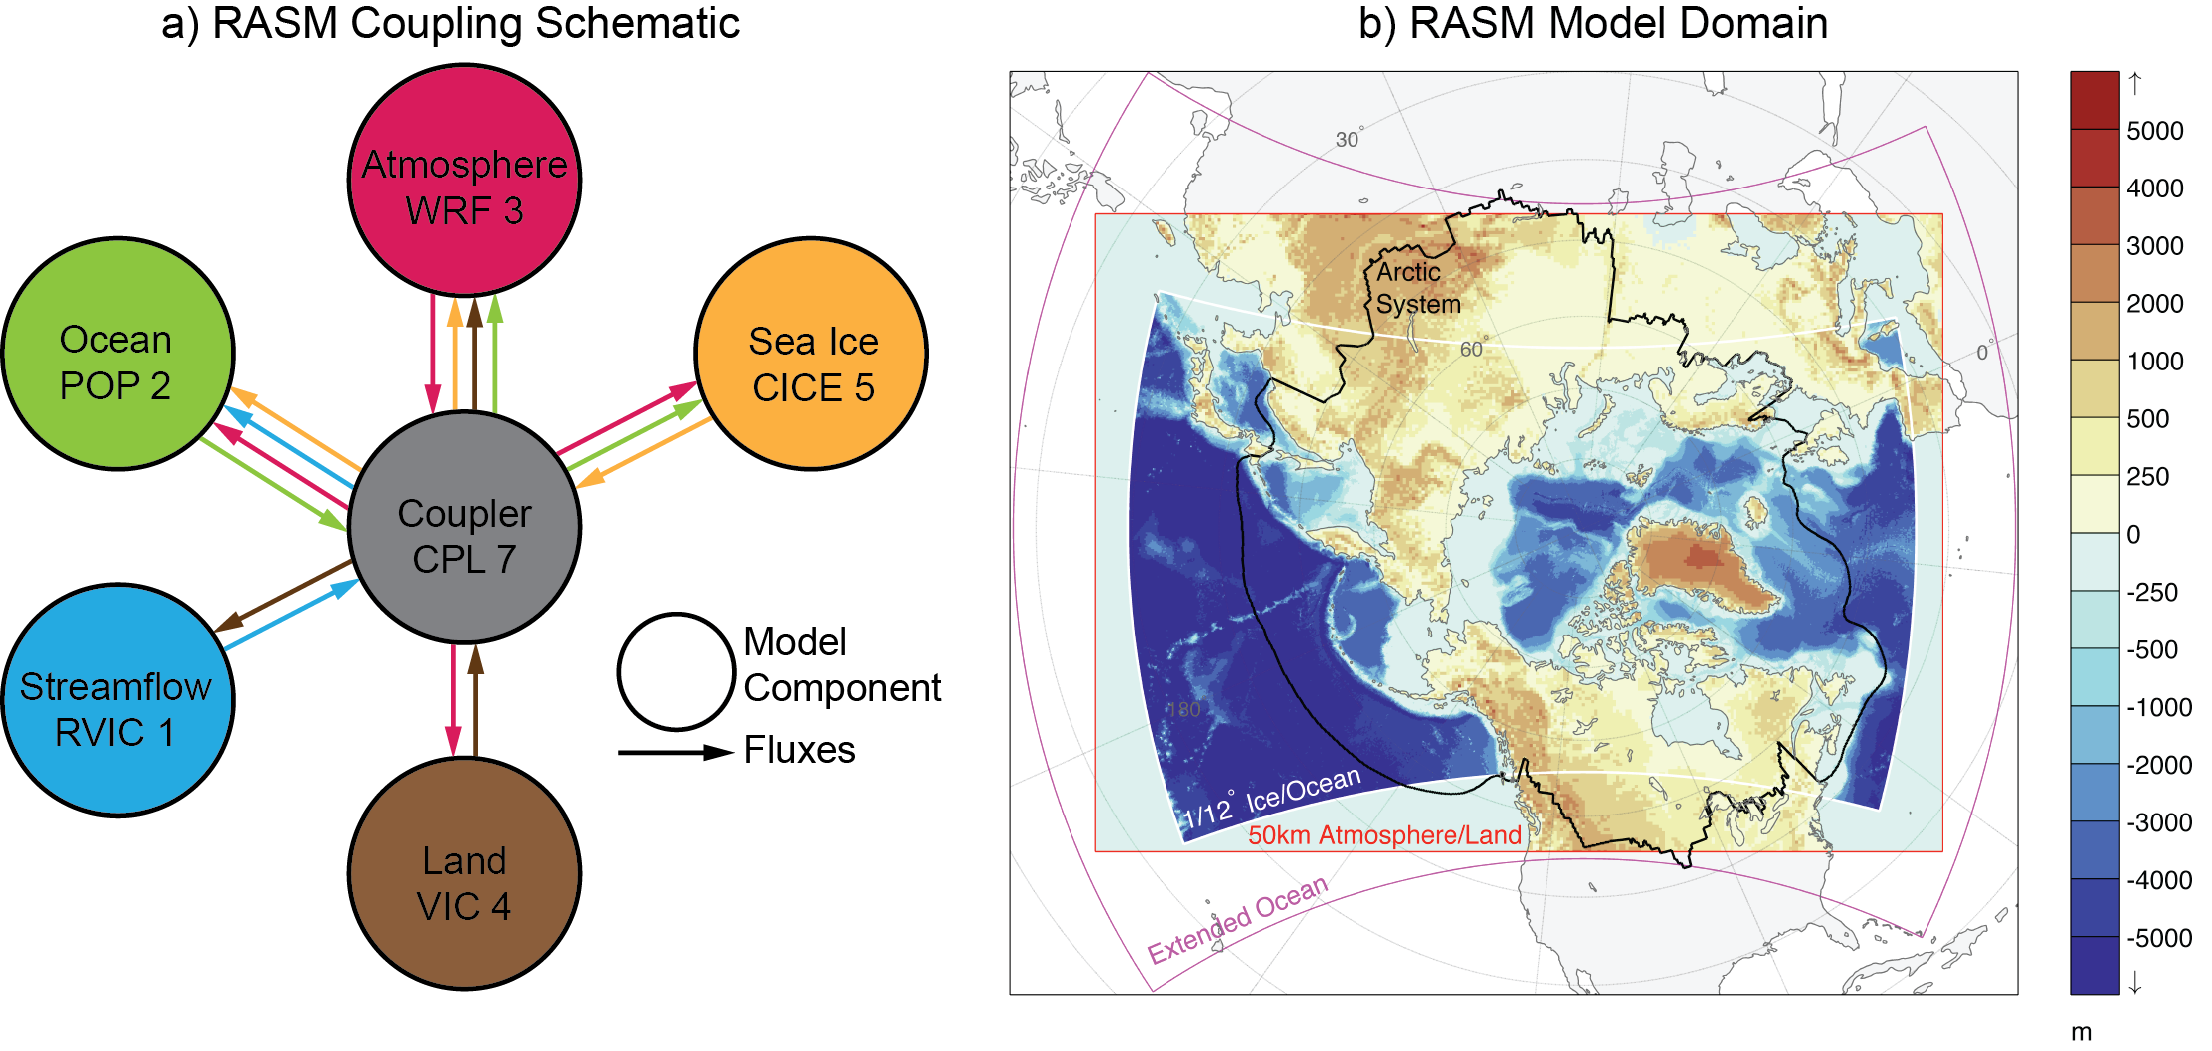
\includegraphics[width=40pc,natwidth=1]{rasm_schematic_domain}
\caption{The Regional Arctic System Model. a) RASM coupling schematic. Circles represent model components and arrows between circles represent flux and state variables shared between components. The colors of the arrows reflect the source of the fluxes and state variables. b) RASM domain, showing the 50-km near equal area domain shared by the land, atmosphere, and streamflow routing components, and the 1/12-degree ocean sea ice domain. TODO: add RVIC drainage area and example basins to b.}
\label{fig:rasm_schematic_domain}
\end{figure}

\clearpage
\begin{figure}
\noindent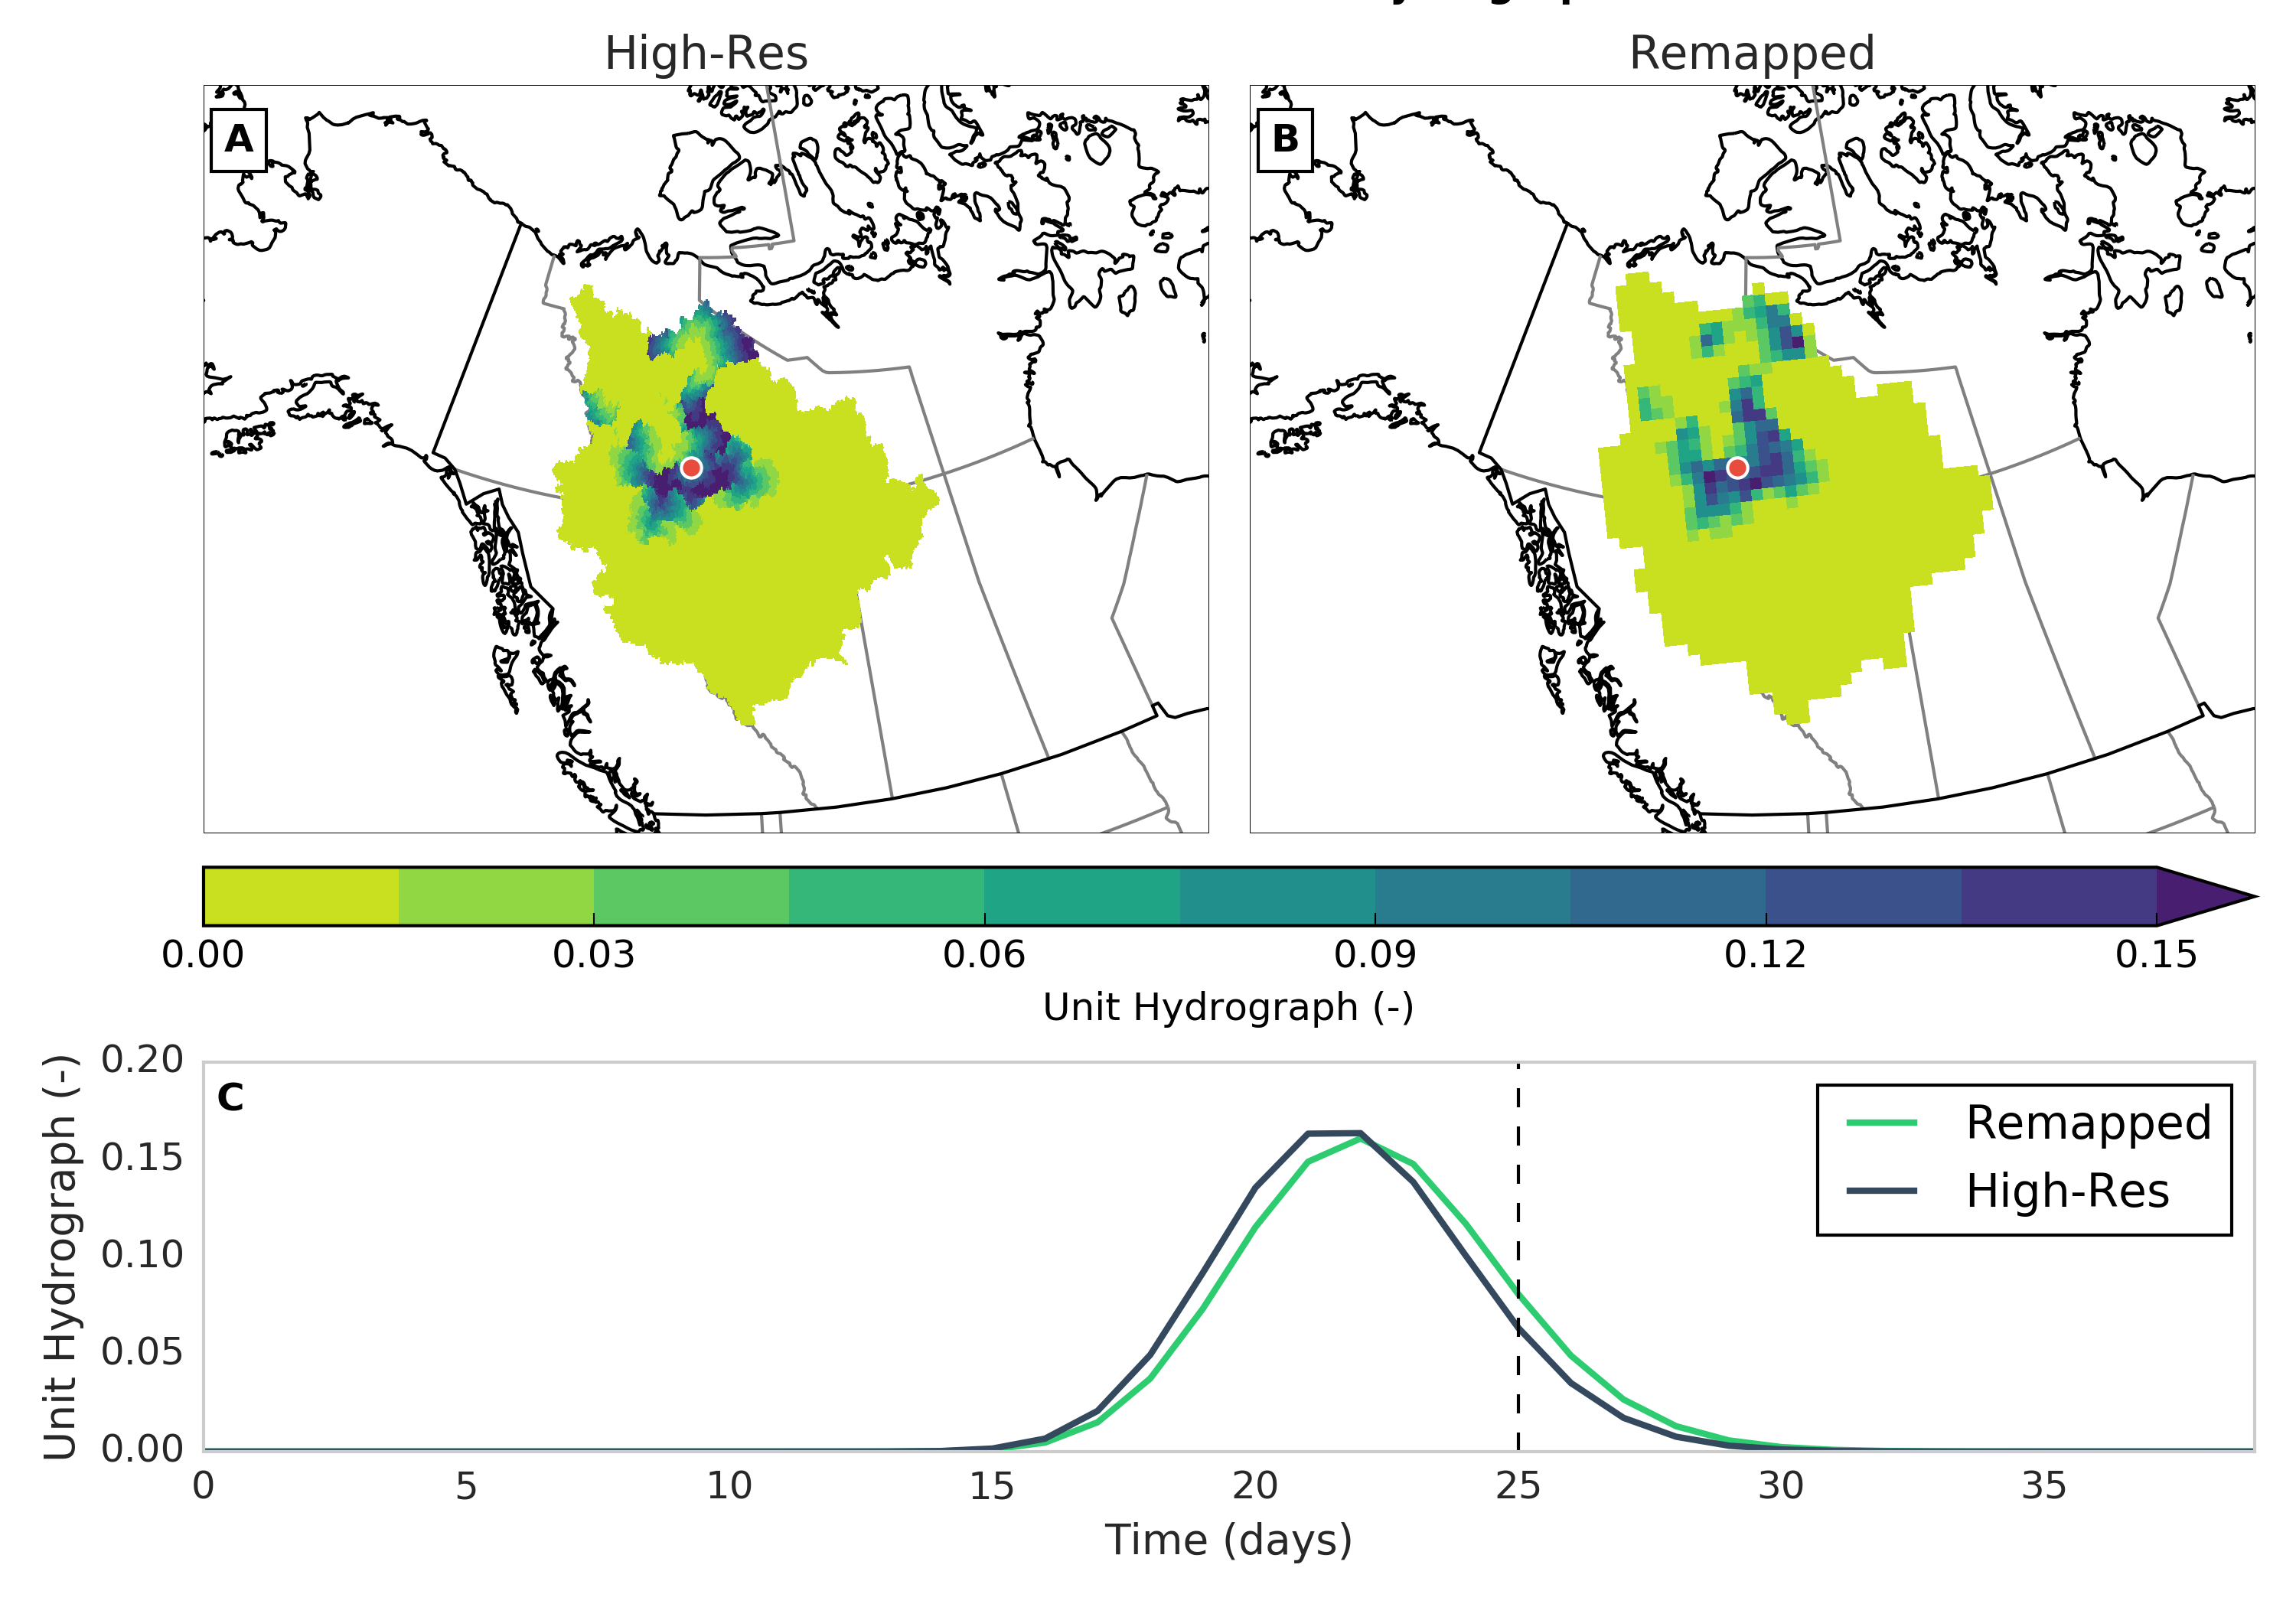
\includegraphics[width=40pc,natwidth=1]{uh_remap_schematic}
\caption{Example of a remapped unit hydrograph grid for the Mackenzie River at Arctic Red River as the outlet location or sink.

This figure depicts the fraction of runoff generated reaching the outlet point on day 25 for the 1/16th degree grid (upper left) and the RASM 50-km grid (upper right). % BN: This sentence is very confusing, please rephrase

The unit hydrographs for the gridcell indicated by the red circle in the center of the basin are shown in the bottom panel.}
\label{fig:uh_remap_schematic}
\end{figure}

\clearpage
\begin{figure}
\noindent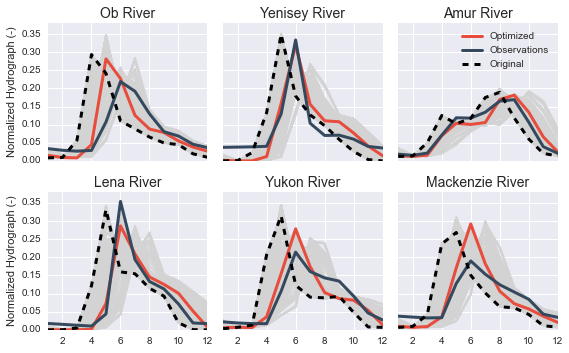
\includegraphics[width=40pc,natwidth=1]{calibration_hydrographs}
\caption{Normalized hydrographs for largest 6 river basins from.  Each trace (grey) represents an individual calibration ensemble member. The observed (normalized) hydrograph for each basin is shown in blue and the hydrograph using the \"Original\" or \"Fast\" parameters is shown in dash-black. TODO: remake this figure with a white background.}
\label{fig:calibration_hydrographs}
\end{figure}

\clearpage
\begin{figure}
\noindent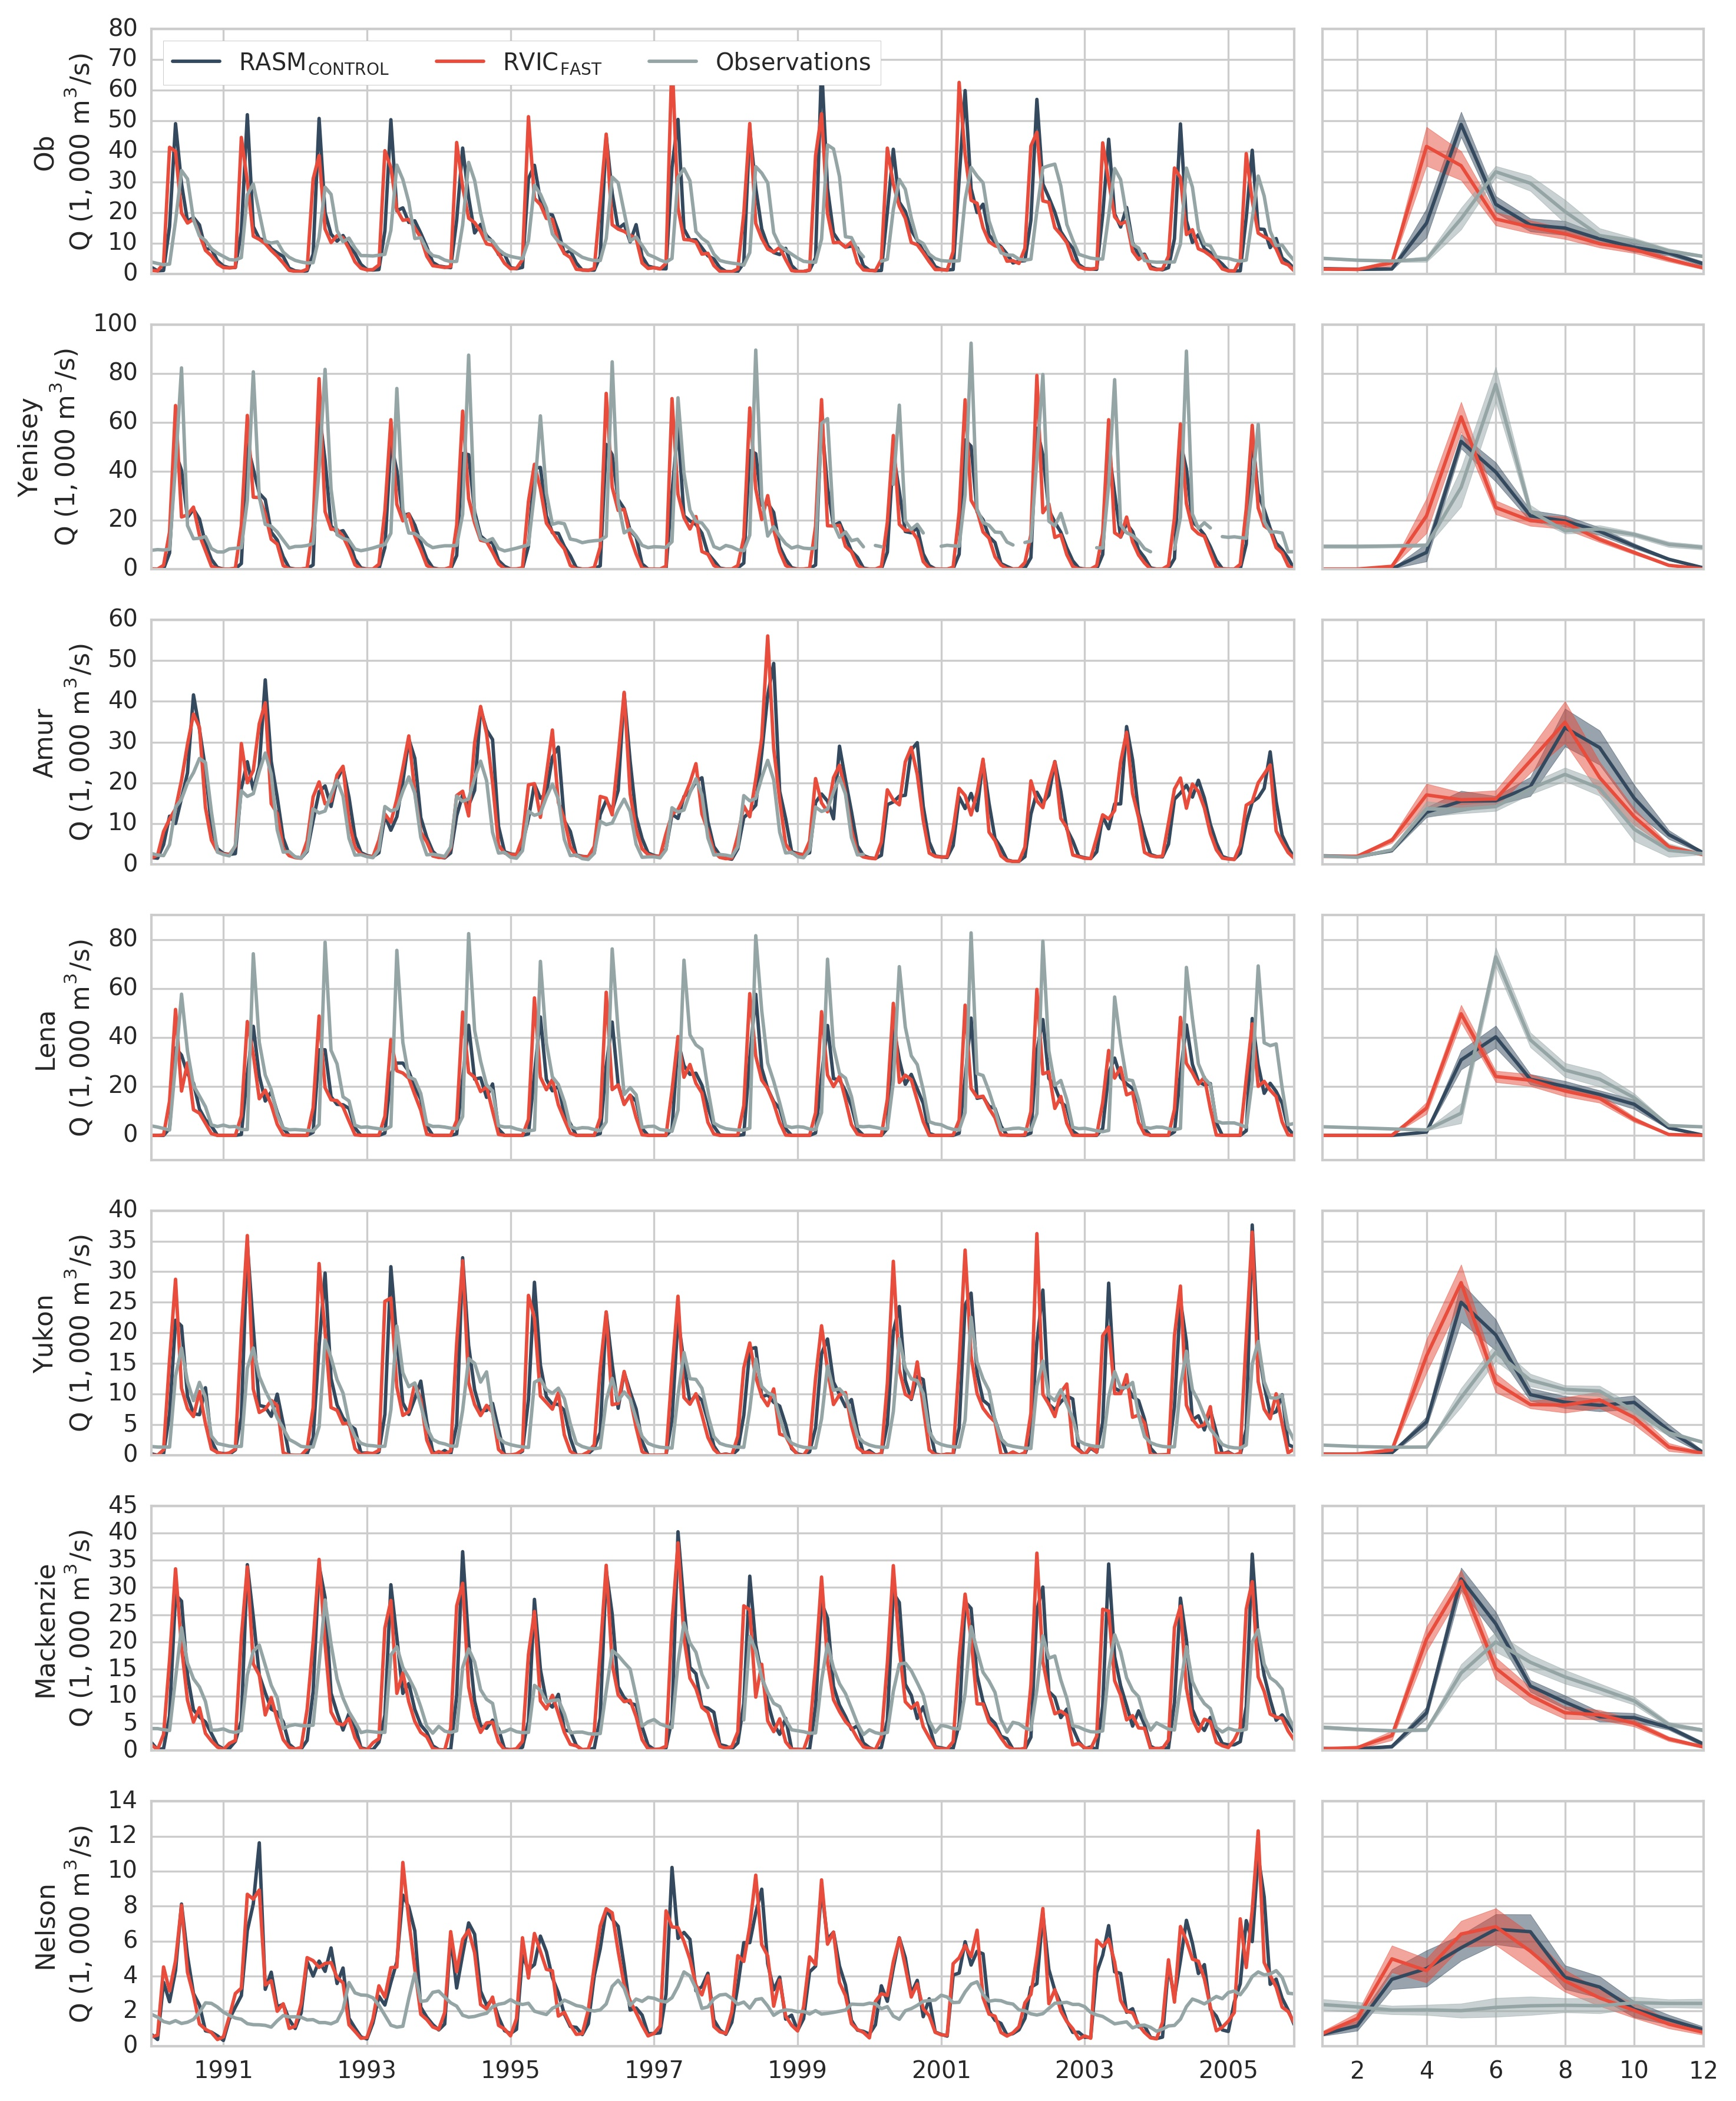
\includegraphics[width=40pc,natwidth=1]{R1010RBRbaaa01a_rvicfast_hydrographs}
\caption{Streamflow hydrographs for the largest 6 river basins compared to values from \citet{Dai_2009}.}
\label{fig:hydrographs}
% BN: Move the basin name for each row into the panel (rather than as part of the Y-axis). For example, in the top right of the right-hand-side panel in each row
% BN: Here and in a number of other figures (4, 6, and 7) I do not like the sequential panel numbering. You have x rows and y columns, not x times y individual plots (which is what the numbering implies). Since you never refer to individual panels (I think), you can remove them. Alternatively, you can use some row.column numbering (A.1, A.2, B.1, B.2, etc)
\end{figure}

\clearpage
\begin{figure}
\noindent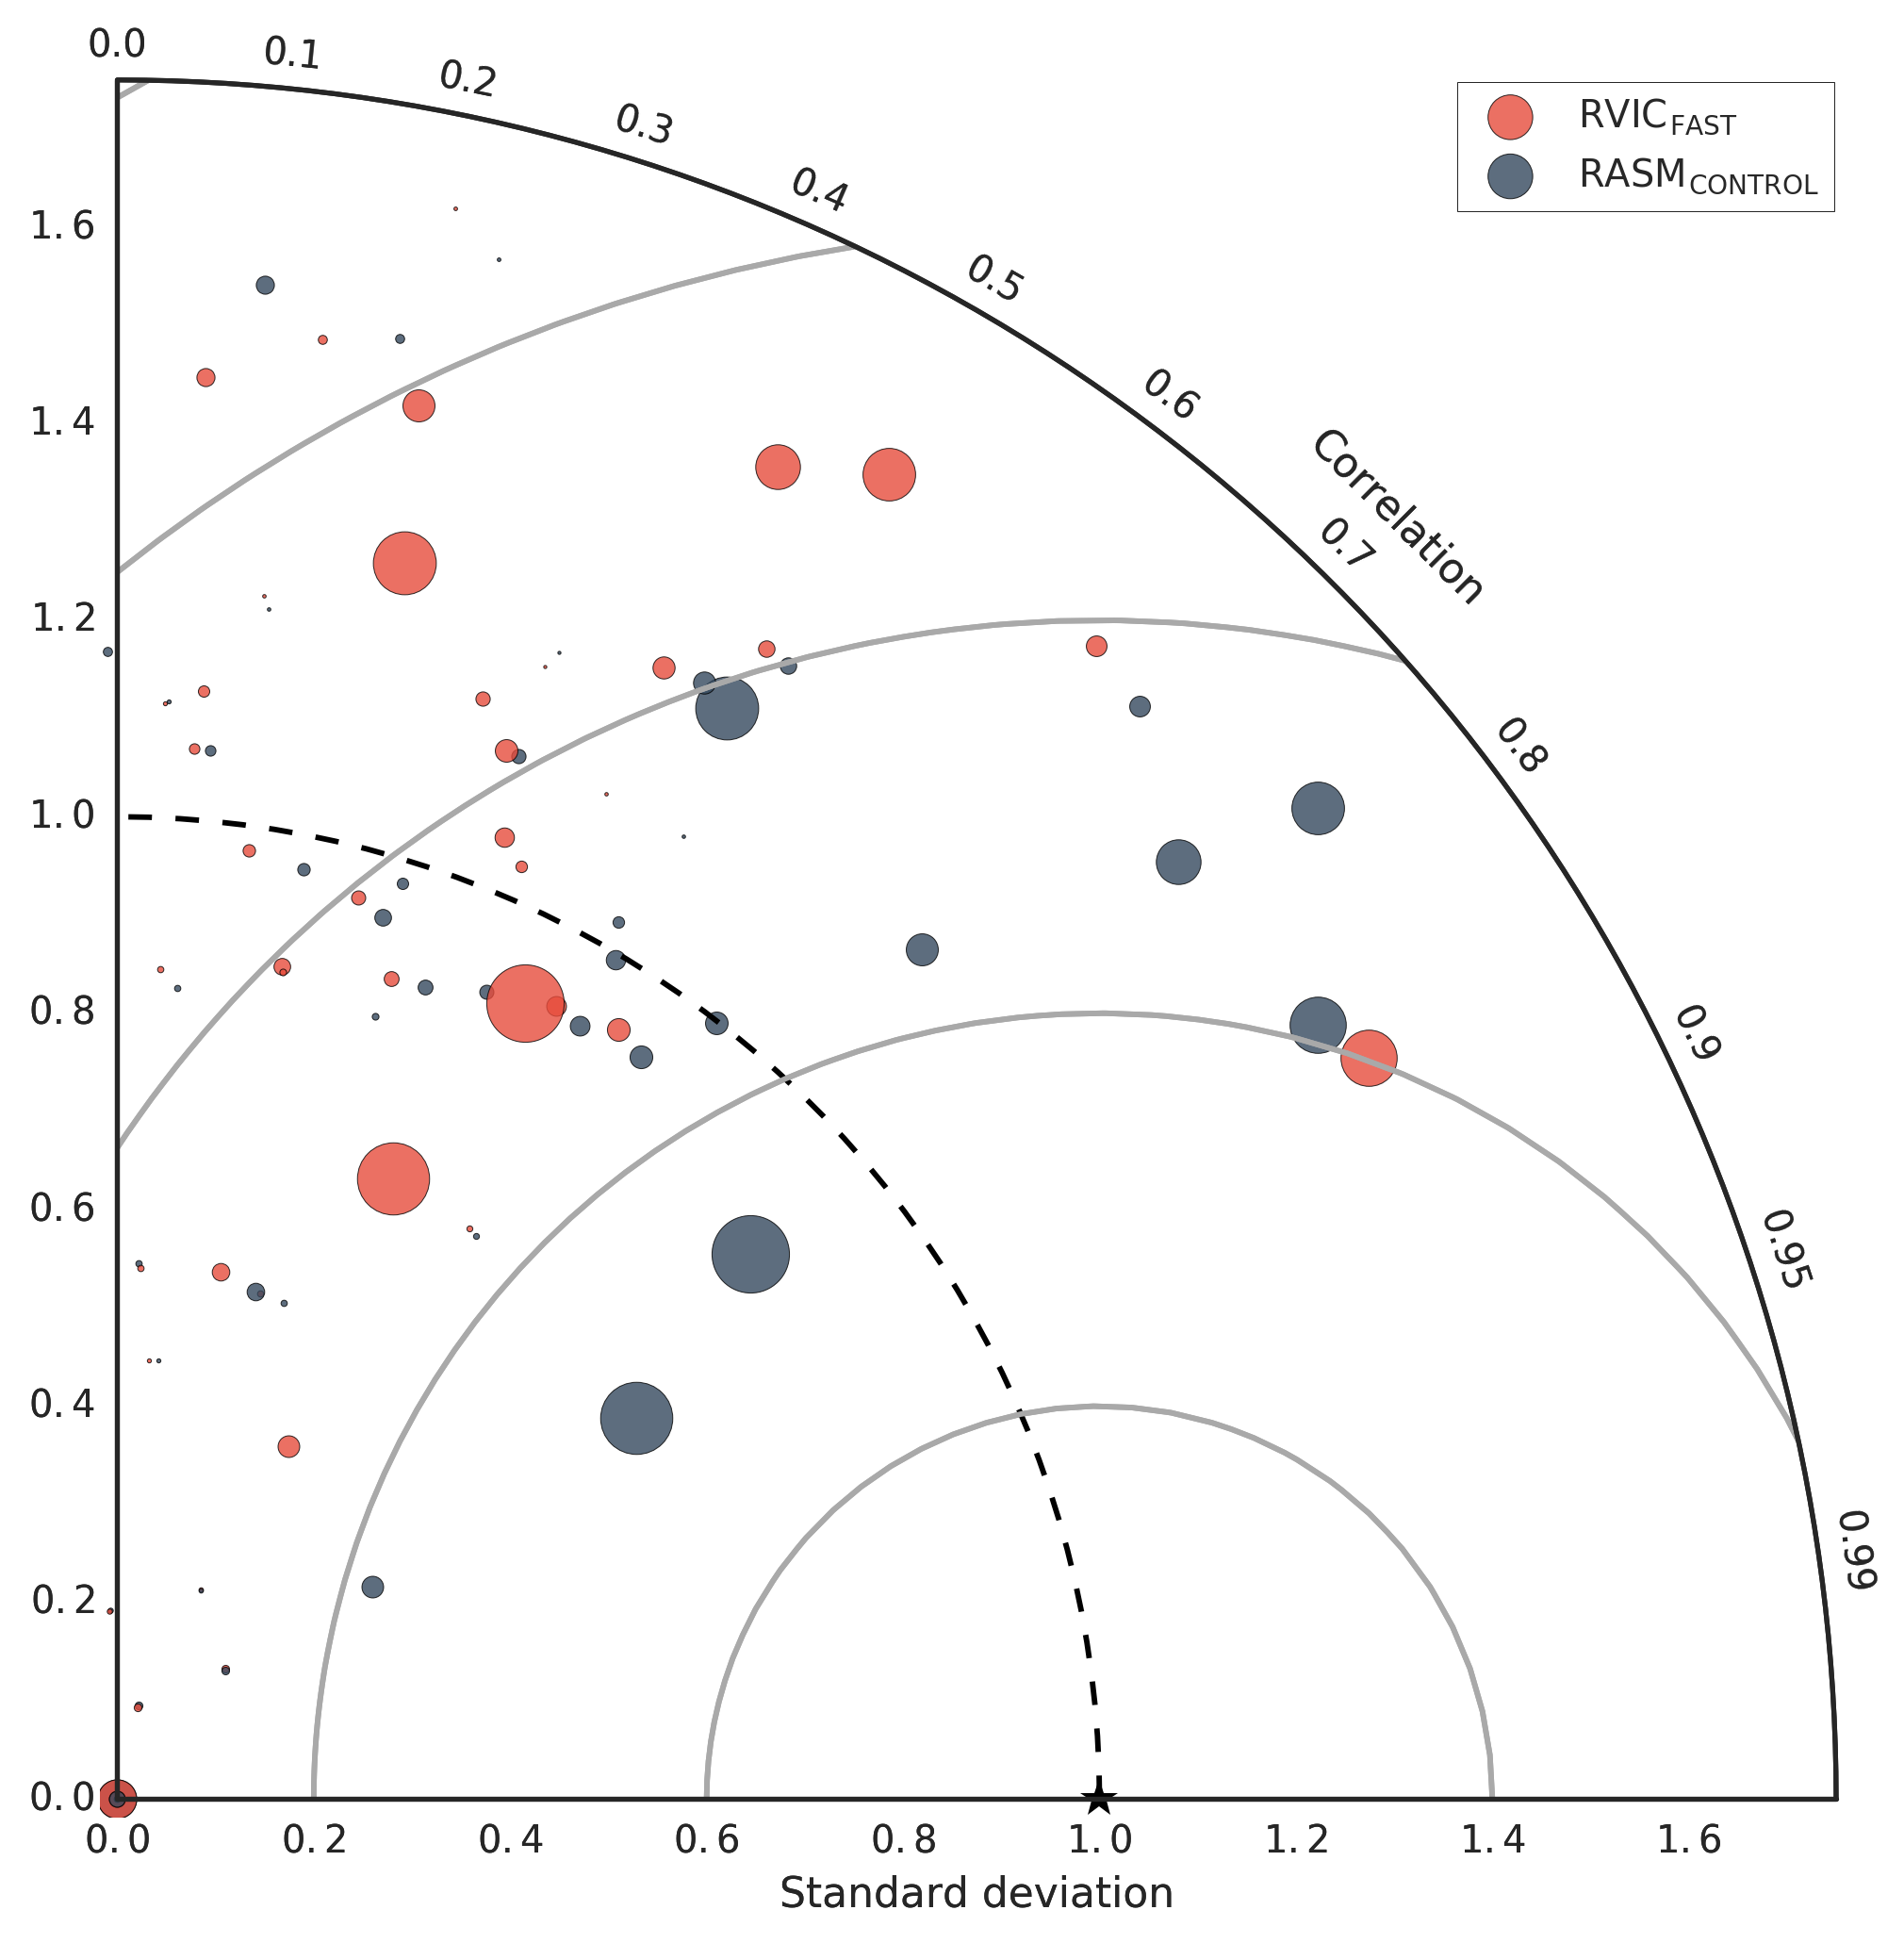
\includegraphics[width=40pc,natwidth=1]{R1010RBRbaaa01a_rvicfast_taylordiag}
\caption{Taylor Diagram showing performance of the RVIC model ($RASM_{CONTROL}$ and $RVIC_{FAST}$) for 64 of the largest rivers in the RASM domain.}
% BN: What is the red circle at (0,0)  -- JJH, not sure, will investigate.
\label{fig:taylor}
\end{figure}

\clearpage
\begin{figure}
\noindent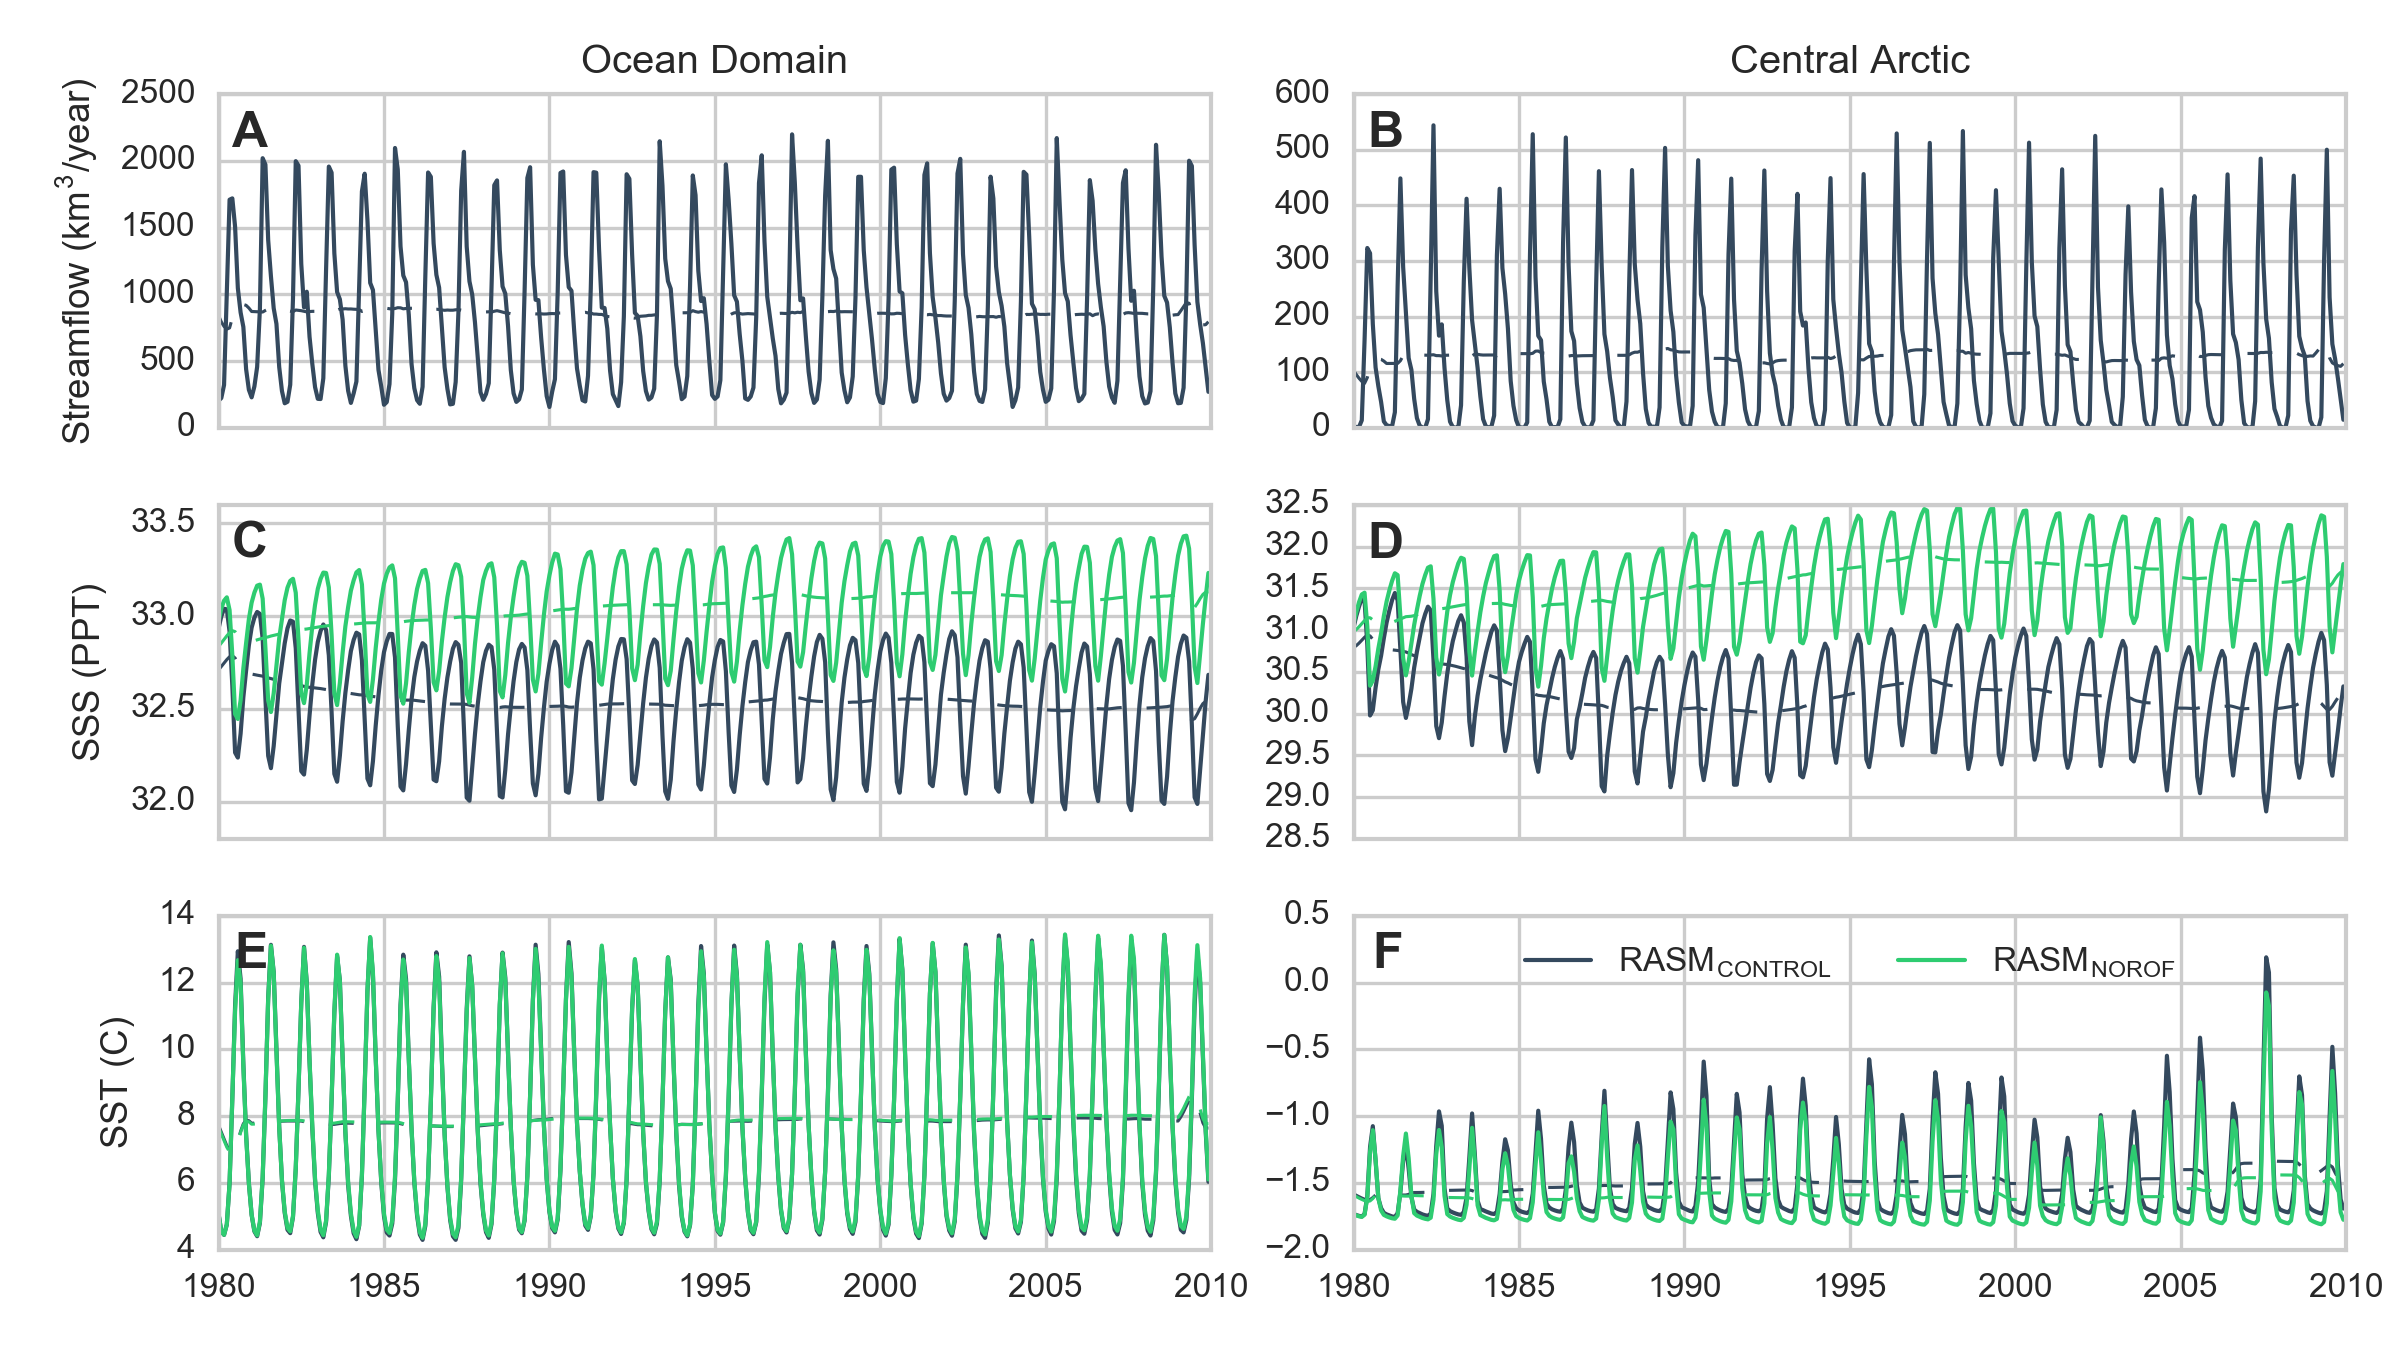
\includegraphics[width=40pc,natwidth=1]{ocean_combine_ts}
\caption{Monthly timeseries (1980-2009) of domain-wide (left) and central arctic (right) streamflow (top), mean SSS (middle), and SST (bottom) for the $RASM_{CONTROL}$ (blue) and $RASM_{NOROF}$ (green). The dashed lines show a 12-month running mean.}
% BN: See comment in figure 4 about labels
% BN: Would it be possible to make a seasonal cycle (like in Figure 4) for the last 20 years, so you can discuss timing effects in more detail?
\label{fig:ocean_timeseries}
\end{figure}

\clearpage
\begin{figure}
\noindent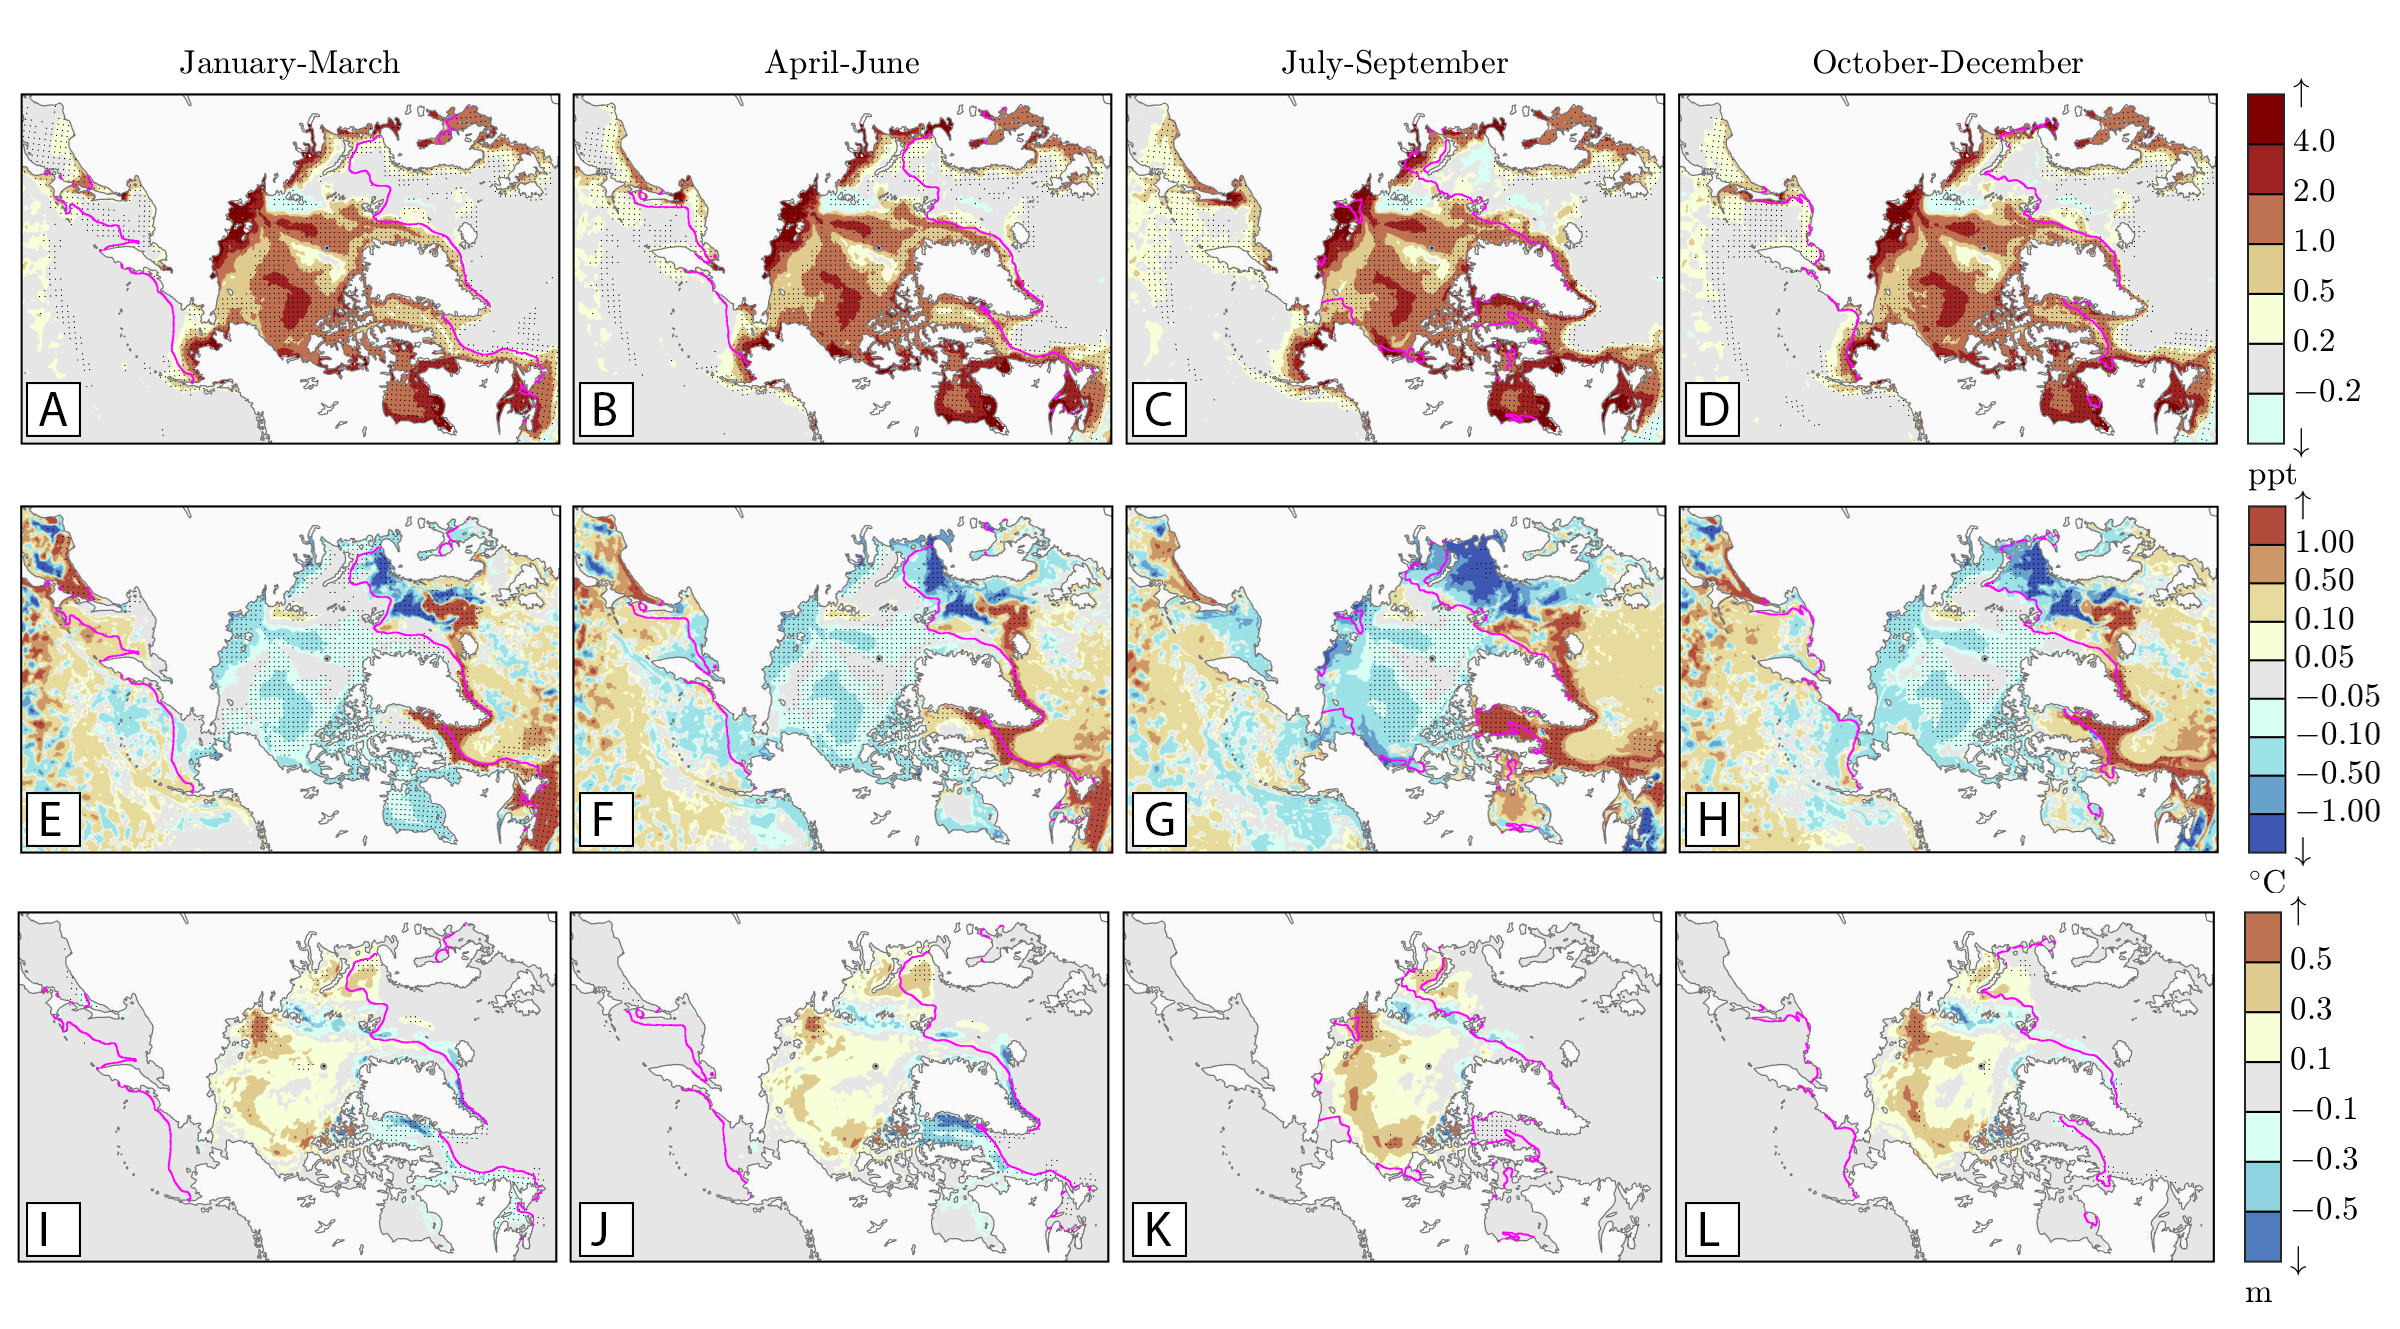
\includegraphics[width=40pc,natwidth=1]{ocean_combine}
\caption{Seasonal difference ($RASM_{NOROF}$ - $RASM_{CONTROL}$) in mean sea surface salinity (top), sea surface temperature (middle), and sea ice height (bottom) (2000-2009). Stippling denotes differences that are statistically significant at the 95 percent confidence interval.}
% BN: See comment in Figure 4 about labels
\label{fig:ocean_maps}
\end{figure}

% Tables
\clearpage

\begin{table}
  \caption{RVIC model performance statistics for the six rivers shown in Figures \ref{fig:calibration_hydrographs} and \ref{fig:hydrographs}.}
  \centering
  \label{table:rivers}
  \resizebox{\textwidth}{!}{%
  \begin{tabular}{|l|c|c|c|c|c|c|}
  {} & \multicolumn{2}{c}{Bias (\%)} & \multicolumn{2}{c}{Overlap (-)}  &  \multicolumn{2}{c}{RMSE ($m^3/s$)} \\
  River & $RASM_{CONTROL}$ & $RVIC_{FAST}$ & $RASM_{CONTROL}$ & $RVIC_{FAST}$ & $RASM_{CONTROL}$ & $RVIC_{FAST}$ \\
  Ob at Salekhard         &            -3.85 &         -3.58 &             0.73 &          0.65 &         12087.04 &      14866.25 \\
  Yenisey at Igarka       &           -25.75 &        -25.81 &             0.75 &          0.64 &         13788.23 &      20114.30 \\
  Amur at Komsomolsk      &            26.85 &         26.66 &             0.90 &          0.93 &          6827.36 &       6711.21 \\
  Lena at Kusur           &           -28.02 &        -28.22 &             0.80 &          0.64 &         13711.20 &      20732.74 \\
  Yukon at Pilot          &            13.21 &         13.35 &             0.79 &          0.66 &          5088.45 &       7359.83 \\
  Mackenzie at Arctic Red &            -4.00 &         -3.79 &             0.75 &          0.67 &          6221.61 &       8215.21 \\
  Nelson at Bladder       &            61.25 &         61.36 &             0.71 &          0.70 &          2878.11 &       2918.71 \\
  \end{tabular}
}
% BN: See comment about bias in text. Also reduce number of significant digits. Reporting RMSE in 100's of liters is incredibly precise, but not at all accurate. I would probably change the units to 100 m3^s and then only provide one number after the decimal. so 2878.11 becomes 28.8 (or thousands and then provide two numbers)
\end{table}

\begin{table}
\caption{Placeholder for table 2}
\centering
\label{table:heat_fluxes}
\begin{tabular}{l c}
\hline
Run  & Time (min)  \\
\hline
 $l1$  & 260   \\
 $l2$  & 300   \\
 $l3$  & 340   \\
 $h1$  & 270   \\
 $h2$  & 250   \\
 $h3$  & 380   \\
 $r1$  & 370   \\
 $r2$  & 390   \\
\hline
\end{tabular}
\tablenotetext{a}{Footnote text here.}
\label{table:2}
\end{table}
\end{document}

%%%%%%%%%%%%%%%%%%%%%%%%%%%%%%%%%%%%%%%%%%%%%%%%%%%%%%%%%%%%%%%

More Information and Advice:

%% ------------------------------------------------------------------------ %%
%
%  SECTION HEADS
%
%% ------------------------------------------------------------------------ %%

% Capitalize the first letter of each word (except for
% prepositions, conjunctions, and articles that are
% three or fewer letters).

% AGU follows standard outline style; therefore, there cannot be a section 1 without
% a section 2, or a section 2.3.1 without a section 2.3.2.
% Please make sure your section numbers are balanced.
% ---------------
% Level 1 head
%
% Use the \section{} command to identify level 1 heads;
% type the appropriate head wording between the curly
% brackets, as shown below.
%
%An example:
%\section{Level 1 Head: Introduction}
%
% ---------------
% Level 2 head
%
% Use the \subsection{} command to identify level 2 heads.
%An example:
%\subsection{Level 2 Head}
%
% ---------------
% Level 3 head
%
% Use the \subsubsection{} command to identify level 3 heads
%An example:
%\subsubsection{Level 3 Head}
%
%---------------
% Level 4 head
%
% Use the \subsubsubsection{} command to identify level 3 heads
% An example:
%\subsubsubsection{Level 4 Head} An example.
%
%% ------------------------------------------------------------------------ %%
%
%  IN-TEXT LISTS
%
%% ------------------------------------------------------------------------ %%
%
% Do not use bulleted lists; enumerated lists are okay.
% \begin{enumerate}
% \item
% \item
% \item
% \end{enumerate}
%
%% ------------------------------------------------------------------------ %%
%
%  EQUATIONS
%
%% ------------------------------------------------------------------------ %%

% Single-line equations are centered.
% Equation arrays will appear left-aligned.

Math coded inside display math mode \[ ...\]
 will not be numbered, e.g.,:
 \[ x^2=y^2 + z^2\]

 Math coded inside \begin{equation} and \end{equation} will
 be automatically numbered, e.g.,:
 \begin{equation}
 x^2=y^2 + z^2
 \end{equation}

% IF YOU HAVE MULTI-LINE EQUATIONS, PLEASE
% BREAK THE EQUATIONS INTO TWO OR MORE LINES
% OF SINGLE COLUMN WIDTH (20 pc, 8.3 cm)
% using double backslashes (\\).

% To create multiline equations, use the
% \begin{eqnarray} and \end{eqnarray} environment
% as demonstrated below.
\begin{eqnarray}
  x_{1} & = & (x - x_{0}) \cos \Theta \nonumber \\
        && + (y - y_{0}) \sin \Theta  \nonumber \\
  y_{1} & = & -(x - x_{0}) \sin \Theta \nonumber \\
        && + (y - y_{0}) \cos \Theta.
\end{eqnarray}

%If you don't want an equation number, use the star form:
%\begin{eqnarray*}...\end{eqnarray*}

% Break each line at a sign of operation
% (+, -, etc.) if possible, with the sign of operation
% on the new line.

% Indent second and subsequent lines to align with
% the first character following the equal sign on the
% first line.

% Use an \hspace{} command to insert horizontal space
% into your equation if necessary. Place an appropriate
% unit of measure between the curly braces, e.g.
% \hspace{1in}; you may have to experiment to achieve
% the correct amount of space.


%% ------------------------------------------------------------------------ %%
%
%  EQUATION NUMBERING: COUNTER
%
%% ------------------------------------------------------------------------ %%

% You may change equation numbering by resetting
% the equation counter or by explicitly numbering
% an equation.

% To explicitly number an equation, type \eqnum{}
% (with the desired number between the brackets)
% after the \begin{equation} or \begin{eqnarray}
% command.  The \eqnum{} command will affect only
% the equation it appears with; LaTeX will number
% any equations appearing later in the manuscript
% according to the equation counter.
%

% If you have a multiline equation that needs only
% one equation number, use a \nonumber command in
% front of the double backslashes (\\) as shown in
% the multiline equation above.

%% ------------------------------------------------------------------------ %%
%
%  SIDEWAYS FIGURE AND TABLE EXAMPLES
%
%% ------------------------------------------------------------------------ %%
%
% For tables and figures, add \usepackage{rotating} to the paper and add the rotating.sty file to the folder.
% AGU prefers the use of {sidewaystable} over {landscapetable} as it causes fewer problems.
%
% \begin{sidewaysfigure}
% \includegraphics[width=20pc]{samplefigure.eps}
% \caption{caption here}
% \label{label_here}
% \end{sidewaysfigure}
%
%
%
% \begin{sidewaystable}
% \caption{}
% \begin{tabular}
% Table layout here.
% \end{tabular}
% \end{sidewaystable}
%
%
